\section{Eulerian Hydrodynamics | Solving PDEs}
\thispagestyle{plain}

As our overarching aim is simulating physical systems (e.g. how do perturbations
evolve in a fluid) and most physical systems are described by partial differential
equations (PDEs) (like the Euler equations), we turn our heads towards numerically solving
PDEs. We search for functions complying to $\mathcal{P}[u] = 0$ (and boundary conditions) with $\mathcal{P}$ being
a differential operator.

\note{This section focuses on solvers following fluid variables on a fixed grid - eulerian hydrodynamics.}

\subsection{Introductory notes on PDEs}
Partial differential equations (like Euler and Navier Stokes equation, Maxwell's equation, ...) describe
relations between partial derivatives of a dependent variable (e.g. fluid density) with respect to
several independent variables (e.g. time and position), like
\begin{equation}
    \partial_t u = \partial_x^2u, \quad \text{dependent variable } u(x,t), \quad \text{independent variables } x,t
\end{equation}
(a kind of 1D diffusion equation).
\note{There is no general approach for solving PDEs.}

\subsection{Types of PDEs}
PDEs are classified by
\begin{itemize}
    \item \textcolor{blue1}{Order of the PDE:} Order of the highest occuring derivative
    \item \textcolor{blue1}{Linearity:} If the dependent variable and all its derivatives only occur linearly (no $\sqrt{\partial_x u}$), the PDE is linear and if $u_1$ and $u_2$ are solutions to the PDE, $c_1u_1+c_2u_2$ are as well (\textcolor{blue1}{superposition})
    \item \textcolor{blue1}{Homogeneity:} The PDE is homogeneous, if all terms contain the dependent variable or its derivatives, so if there is no source term
\end{itemize}

\subsubsection{Classification of linear 2nd order PDEs in analogy with conic sections}
PDEs can be distinguished into different types which give clues about appropriate solution strategies
as well as appropriate initial and boundary conditions and the smoothness of the solution.

Consider a 2nd order linear PDE with two independent variables, so generally

\begin{equation}
    a \frac{\partial^2 u}{\partial x^2}+b \frac{\partial^2 u}{\partial x \partial y}+c \frac{\partial^2 u}{\partial y^2}+d \frac{\partial u}{\partial x}+e \frac{\partial u}{\partial y}+f u=g, \quad a, b, c \text { not all zero }
\end{equation}

\subsubsubsection{Derivation | homogeneous solutions are conic section in $k$-space}
The unknown function $u$ is expanded into plane waves (Fourier transformation)
\begin{equation}
    u(\vec{x})=\frac{1}{(2 \pi)^2} \int \hat{u}(\vec{k}) \exp (-i\vec{k} \cdot \vec{x}) d^2 k, \quad \vec{k}=:\left(\begin{array}{c}
    k \\
    l
    \end{array}\right)
\end{equation}
Plugging this into the PDE yields
\begin{equation}
    -\frac{1}{(2\pi)^2} \int{\left(\mathcolor{red1}{ak^2+bkl+cl^2+idk+idk-f}\right) \hat{u}(\vec{k}) \exp{(-i\vec{k}\cdot \vec{x})}} d^2k = g
\end{equation}
For the homogeneous solution ($g = 0$) \textcolor{red1}{this} must be zero, so
\begin{equation}
    \vec{k}^T \mat{\Delta} \vec{k} + i \begin{pmatrix}d \\ e\end{pmatrix}^T \vec{k} - f = 0, \quad \mat{\Delta} = \begin{pmatrix} a & b/2 \\ b/2 & c\end{pmatrix}
\end{equation}
which is the matrix representation of a conic section in $\vec{k}$-space (why?).

\subsubsubsection{Classification into elliptic, parabolic, hyperbolic}
\begin{equation}
    \text { The PDE is }\left\{\begin{array}{c}
    \text { hyperbolic if } D>0 \\
    \text { parabolic if } D=0, \\
    \text { elliptic if } D<0
    \end{array} \quad \Delta=\left|\begin{array}{cc}
    a & b / 2 \\
    b / 2 & c
    \end{array}\right|, \quad D=-4 \Delta=b^2-4 a c\right.
\end{equation}

\subsubsubsection{Qualitative differences of the types of PDEs}
\begin{itemize}
    \item \textcolor{blue1}{Elliptic}
    \begin{itemize}
        \item often describe static problems (no time dependence) like 
        the Poisson equation ($\vec{\nabla}^2\phi = -\frac{\rho}{\epsilon}$)
        \item as smooth as coefficients allow in the interior region where the equation and solutions are defined (independent of the smoothness of the boundary conditions)
    \end{itemize}
    \item \textcolor{blue1}{Parabolic}
    \begin{itemize}
        \item often of second order, describing slowly changing processes like diffusion, becoming smoother with time
        \item the problem is described using an initial state $u(x,t_0)$ as well as boundary conditions
        \item all parabolic PDEs can be transformed into a form analogous to the heat equation by change of independent variables
    \end{itemize}
    \item \textcolor{blue1}{Hyperbolic}
    \begin{itemize}
        \item typically describe dynamical processes in physics
        \item initial conditions are specified by $u(x,t_0), \frac{\partial u}{\partial x}(x,t_0)$ and higher derivatives as necessary as well as boundary conditions
        \item disturbances have finite propagation speed
        \item solutions can develop steep regions and real discontinuities
    \end{itemize}
\end{itemize}



\textcolor{blue1}{Boundary types:} Fixed function values on the boundaries $=$ Dirichlet boundary; fixed value of the derivative $=$ van Neumann boundary.

\subsubsection{Typical examples and classification of homogeneous 2nd order PDEs}

\begin{table}[!htb]
    \centering
    \begin{tabular}{|p{0.5\textwidth}|p{0.5\textwidth}|}
    \hline
    \textcolor{blue1}{Equation} & \textcolor{blue1}{Classification} \\
    \hline
    \hline
    Laplace equation
    \begin{equation}
        \begin{gathered}
            \vec{\nabla}^2 u = \partial_x^2 u + \partial_y^2 u = 0 \\
            (a = 1, b = 0, c = 1)
        \end{gathered}
    \end{equation} & Elliptic \\
    \hline
    1D Heat conduction equation (diffusion equation)
    \begin{equation}
        \begin{gathered}
            \partial_t u - \lambda^2 \partial_x^2 u = 0 \\
            (a = 0, b = 0, d = 1, c = -\lambda^2)
        \end{gathered}
    \end{equation} & Parabolic \\
    \hline
    1D Wave equation
    \begin{equation}
        \begin{gathered}
            \partial_t^2 u - c_s^2 \partial_x^2 u = 0 \\
            (a = 1, b = 0, c = -c_s^2)
        \end{gathered}
    \end{equation} & Hyperbolic \\
    \hline
    \end{tabular}
    \caption{Typical examples and classification of homogeneous 2nd order PDEs}
    \label{tab:2nd_order_pdes}
\end{table}

\note{The classification scheme introduced is for 2nd order PDEs with two variables, it is not made e.g. for the advection equation $\partial_t u + v \partial_x u = 0$ which is first order and hyperbolic.}

\subsubsection{Classification of linear 2nd order PDEs with more unknowns}
For the general form
\begin{equation}
    \sum_{i, j=1}^n A_{i j} \frac{\partial^2 u}{\partial x_i \partial x_j}+\sum_{i=1}^n b_i \frac{\partial u}{\partial x_i}+c u+d=0, \quad \mat{A} \text { with entries } A_{i j}
\end{equation}
regarding the eigenvalues of $\mat{A}$ (following from $\mat{A}\vec{v} = \lambda \vec{v} \rightarrow \det(\mat{A}-\lambda \mat{I}) = 0$) it holds that
\begin{equation}
    \text { The PDE is }\left\{\begin{array}{c}
    \text { hyperbolic if one negative, rest postitive or one positive, rest negative } \\
    \text { parabolic if one zero, others all positive or all negative } \\
    \text { elliptic if all positive or all negative }
    \end{array}\right.
\end{equation}
Note that this classification is not exhaustive, the occurrence of multiple different signs is sometimes called ultra-hyperbolic.

Task to the reader: Check that for $n=2$ this classification scheme is equivalent to the previous one.

\subsubsection{Linear systems of 1st order homogeneous PDEs}
\greenbox{\textbf{Question:} When is a 1st order homogeneous PDE hyperbolic?}
A first order homogeneous PDE is of the form
\begin{equation}
    \partial_t u_i + \sum_{j=1}^n A_{i j} \partial_{x_j} u_i = 0, \quad i = 1, \dots, n
\end{equation}
with short-hand notation
\begin{equation}
    \partial_t \vec{u} + \left(\mat{A} \mat{\nabla}_\vec{x} \right) \vec{u} = 0, \quad \mat{A} \text { with entries } A_{i j}, \quad \mat{\nabla}_\vec{x} = \text{diag}(\partial_{x_1}, \dots, \partial_{x_n})
\end{equation}
where \textbf{the system is hyperbolic if $\mat{A}$ has real eigenvalues and is diagonizable}.
\subsubsubsection{Extension to conservation laws}
We extend this to conservation laws
\begin{equation}
    \partial_t \vec{u} + \vec{\nabla}_\vec{x} \cdot \mat{F}(\vec{u}) = \partial_t \vec{u} + (\mat{\nabla}_\vec{u} \mat{F}(\vec{u})) \mat{\nabla}_\vec{x} \vec{u} = 0
\end{equation}
with conserved variable $\vec{u}$ and flux matrix $\mat{F}(\vec{u})$. IF $\mat{\nabla}_\vec{u} \mat{F}(\vec{u})$ is diagonizable with real eigenvalues, the system is hyperbolic.

Consider e.g. the Navier-Stokes equation

\begin{equation}
    \partial_t (\rho \vec{v}) + \vec{\nabla} \cdot (\rho \vec{v} \vec{v}^T + P \mat{I} - \mat{\Pi}) = \rho \vec{g}
\end{equation}

where $\vec{\nabla} \cdot$ here is a matrix divergence (a vector) with entries as expected for such a matrix vector multiplication.
\note{The classification introduced has its limits: What type the Navier-Stokes equation
is seems different to tell, often \textit{hyperbolic} is used as \textit{advection-dominated} (the advection equation is hyperbolic) and \textit{parabolic} as \textit{diffusion-dominated} (the diffusion equation is parabolic) and then the Navier
stokes equation can be either depending on the Reynolds number.}

\bluebox{\textbf{Solving an elliptic problem by solving a hyperbolic problem to steady state\skipthis:}
Consider for instance the elliptic Poisson equation
\begin{equation}
    \vec{\nabla}^2 \phi = 4\pi G \rho
\end{equation}
from which hyperbolic gravity equations can be obtained as
\begin{equation}
    \begin{gathered}
        \frac{\partial}{\partial \tau}\left[\begin{array}{c}
            \phi \\
            q_1 \\
            q_2
            \end{array}\right]+\frac{\partial}{\partial x}\left[\begin{array}{c}
            -q_1 \\
            -\phi / T_r \\
            0
            \end{array}\right]+\frac{\partial}{\partial y}\left[\begin{array}{c}
            -q_2 \\
            0 \\
            -\phi / T_r
            \end{array}\right]=\left[\begin{array}{l}
            -4 \pi G \rho \\
            -q_1 / T_r \\
            -q_2 / T_r
            \end{array}\right], \quad \left( \begin{array}{c}
                q_1 \\ q_2
            \end{array} \right) \approx \vec{\nabla} \phi  \\
            \text{pseudotime } \tau, \text{ relaxation time } T_r
    \end{gathered}
\end{equation}
which can then be used in the (compressible) Euler equations
\begin{equation}
    \begin{gathered}
        \frac{\partial}{\partial t}\left[\begin{array}{c}
            \rho \\
            \rho v_1 \\
            \rho v_2 \\
            E
            \end{array}\right]+\frac{\partial}{\partial x}\left[\begin{array}{c}
            \rho v_1 \\
            \rho v_1^2+p \\
            \rho v_1 v_2 \\
            (E+p) v_1
            \end{array}\right]+\frac{\partial}{\partial y}\left[\begin{array}{c}
            \rho v_2 \\
            \rho v_1 v_2 \\
            \rho v_2^2+p \\
            (E+p) v_2
            \end{array}\right]=\left[\begin{array}{c}
            0 \\
            -\rho \partial_x\phi \\
            -\rho \partial_y\phi \\
            -(\vec{v} \cdot \vec{\nabla} \phi) \rho
            \end{array}\right] \\
            p = (\gamma-1)\left(E-\frac{1}{2}\rho (v_1^2 + v_2^2)\right)
    \end{gathered}
\end{equation}
to evolve a self-gravitating fluid only using a hyperbolic solver (e.g. a purely hyperbolic
discontinuous Galerkin approach as in \cite{schlottke21}).
}

\subsection{Solution schemes for PDEs}
There is no general approach but mutltiple general
methods for different types or even only a certain PDE.
Common methods are
\begin{itemize}
    \item \textcolor{blue1}{Finite difference methods:} Differential operators are approximated by finite difference operators, usually on a regular (Cartesian) mesh
    \item \textcolor{blue1}{Finite volume methods:} Useful for hyperbolic conservation 
    laws. We consider quantities averaged over finite volumes around mesh cells where 
    divergence terms in a PDE turn into fluxes through the cells surface ($\rightarrow$ conservative 
    method, fluxes are not lost). Exact expressions for the average value of the solution over some volumes 
    are calculated and from these averages solutions within the cells can be reconstructed. This \textbf{contrasts with 
    finite difference methods where derivatives are approximated based on nodal values and finite element 
    methods where local approximations are made using local data} and stitched together to a global solution.
    \item \textcolor{blue1}{Spectral methods:} The PDE is converted into an algebraic form (e.g. by Fourier transform), the solution is represented by a linear combination of functions (e.g. the plane waves from the inverse Fourier transform).
    \item \textcolor{blue1}{Method of lines:} All derivatives but one are approximated by finite differences, leading to an ODE system, where we can use ODE solvers. \textbf{Time-dependent problems:} Consider a time-dependent problem on a 1D grid, $x_i, i=1,...,N$. Each point yields and ODE for the time evolution of the solution at that point, dependent on e.g. the solution on neighboring points $\rightarrow$ $N$ coupled ODEs.
    \item \textcolor{blue1}{Finite element methods:} The simulation domain is divided into cells (elements, arbitrary shape, unstructured mesh) and the solution on each cell approximated in form of a simple (polynomial) function. The solutions from the cells are linearly combined and we solve for the coefficients.
\end{itemize}

\textcolor{blue1}{Example for the method of lines: } Consider the 1D heat equation
\begin{equation}
    \partial_t u - \lambda^2 \partial_x^2 u = 0
\end{equation}
\greenbox{\textbf{How to discretize the 2nd order derivative $\partial_x^2 u$?}: Second order Taylor expansion yields
\begin{equation}
    \begin{aligned}
        u(x+\Delta x) &= u(x) + \Delta x \partial_x u(x) + \frac{1}{2} \Delta x^2 \partial_x^2 u(x) + \mathcal{O}(\Delta x^3) \\
        u(x-\Delta x) &= u(x) - \Delta x \partial_x u(x) + \frac{1}{2} \Delta x^2 \partial_x^2 u(x) + \mathcal{O}(\Delta x^3)
    \end{aligned}
\end{equation}
where adding both yields
\begin{equation}
    \label{eq:2nd_disc}
    \partial_x^2 u(x) \approx \frac{u(x+\Delta x) - 2u(x) + u(x-\Delta x)}{\Delta x^2}
\end{equation}
}
We therefore get
\begin{equation}
    \partial_t u_i - \lambda^2 \frac{u_{i+1} - 2u_i + u_{i-1}}{h^2} = 0, \quad i = 1, \dots, N
\end{equation}
which we could for instance approach using the Euler method. The grid is illustrated in fig. \ref{fig:method_of_lines_grid}.
\begin{figure}[htb!]
    \centering
    \includesvg[width=0.8\textwidth]{figures/method_of_lines_grid.svg}
    \caption{1D grid}
    \label{fig:method_of_lines_grid}
\end{figure}

\problem{This scheme might not be stable.}

\subsection{Advection - Keep information flow in the physical system in mind}
Consider the first-order hyperbolic advection equation
\begin{equation}
    \partial_t u + v \partial_x u = 0, \text{we seek } u(x,t), \quad v \text{ constant parameter}
\end{equation}
which is hyperbolic as of the real and \textit{diagonizable} coefficient matrix (a scalar).
\subsubsubsection{Analytic solution to the advection equation}
For any function $q(x)$, the function $u(x,t) = q(x-vt)$ is a solution to the advection equation ($\partial_t u = -v \partial_x q$) (see fig. \ref{fig:advection}).

\begin{figure}[htb!]
    \centering
    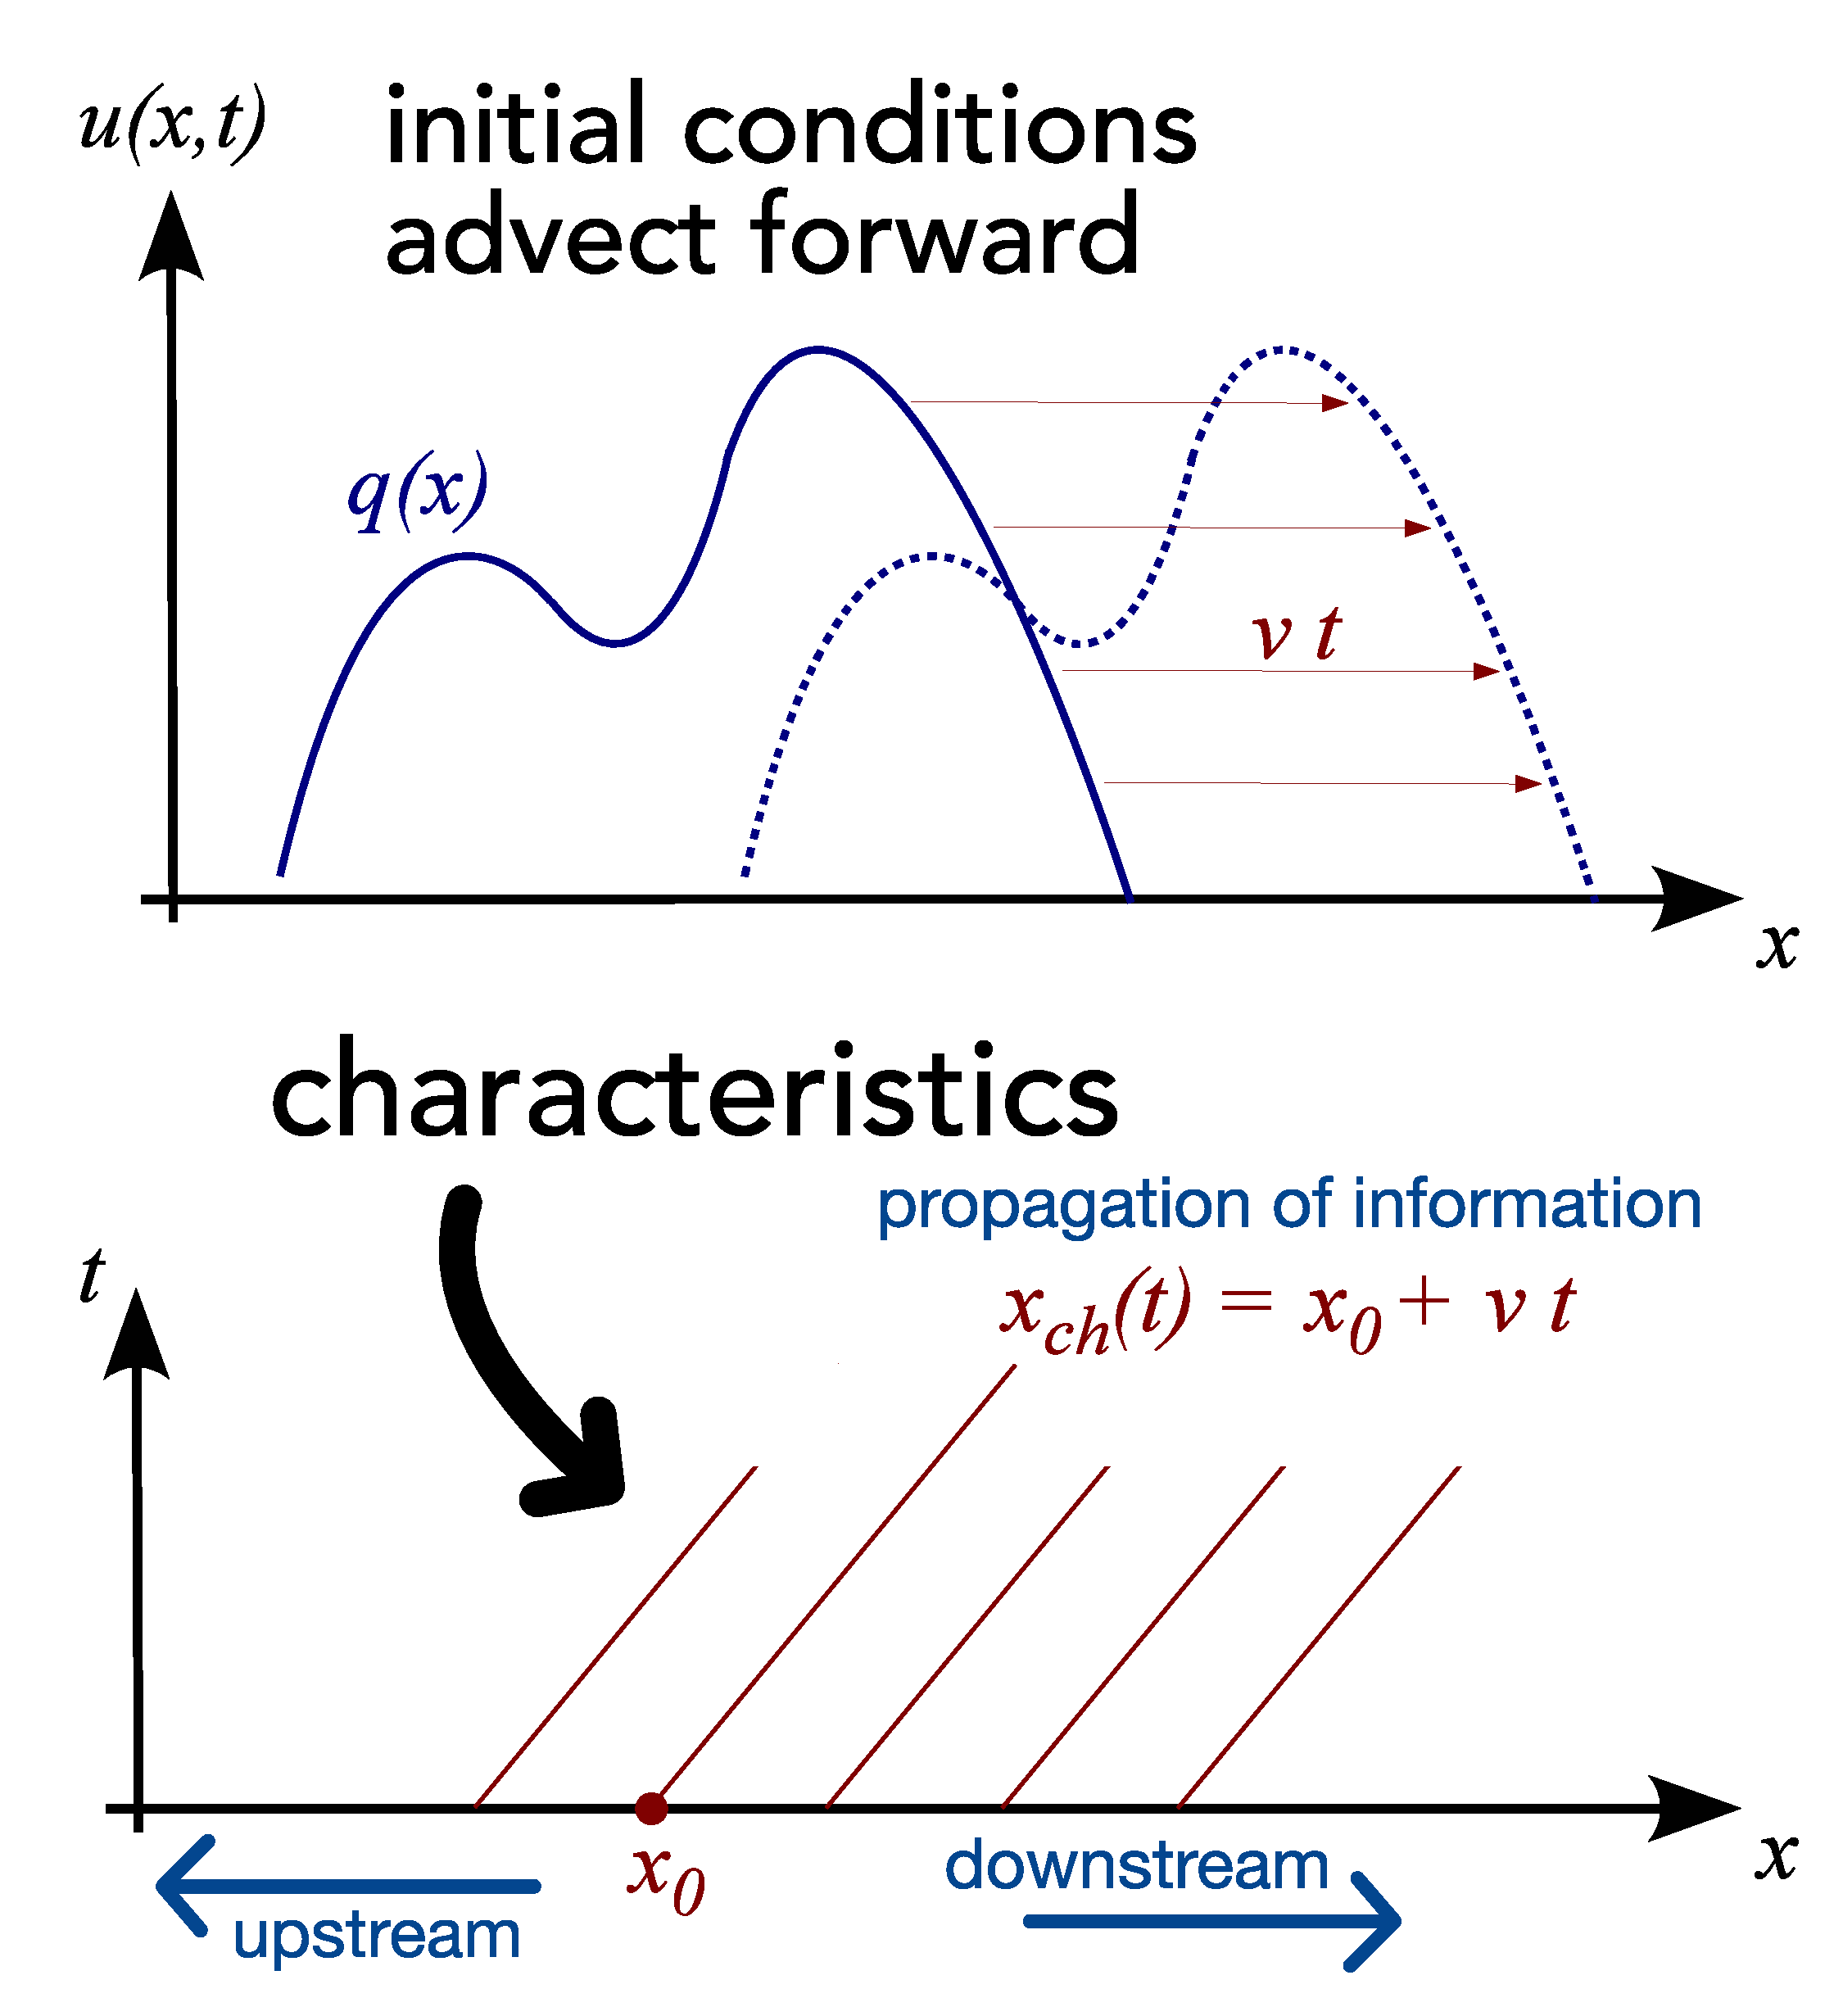
\includegraphics[width=0.8\textwidth]{figures/advection.pdf}
    \caption{Advection}
    \label{fig:advection}
\end{figure}

Interpreting $u(x,t = 0) = q(x)$ as an initial condition, the solution at a later time is just a shifted (by $vt$ along $x$) copy of $q(x)$.

While for the advection problem we know the analytic solution, it helps us uncover the basic cavets of numerically solving PDEs.

\subsubsubsection{Simple but wrong approach | we need to consider the flow of information}
Let us replace the derivative in space by a central difference with respect to the neighboring grid points
\begin{equation}
    \frac{\partial u_i}{\partial t}+v \frac{u_{i+1}-u_{i-1}}{2 h}=0
\end{equation}
and step in time using explicit Euler
\begin{equation}
    u_i^{(n+1)}=u_i^{(n)}-v \frac{u_{i+1}^{(n)}-u_{i-1}^{(n)}}{2 h} \Delta t
\end{equation}
\problem{This is violently unstable (illustrated in \ref{fig:advection_unstable}), as (based on the characteristics) information should only travel downstream but in the central differencing, we use upstream information $u_{i+1}^{(n)}$}

\begin{figure}[htb!]
    \centering
    \includesvg[width=0.8\textwidth]{figures/advection_unstable.svg}
    \caption{Advection with central differencing, violently unstable}
    \label{fig:advection_unstable}
\end{figure}

\subsubsubsection{Directional splitting / upwind scheme to the rescue}
Let us only use upstream information, so (mind the sign of $v$)
\begin{equation}
    \begin{aligned}
        v > 0&: u_i^{(n+1)} = u_i^{(n)} - v \frac{u_i^{(n)} - u_{i-1}^{(n)}}{h} \Delta t  \\
        v < 0&: u_i^{(n+1)} = u_i^{(n)} - v \frac{u_{i+1}^{(n)} - u_{i}^{(n)}}{h} \Delta t 
    \end{aligned}
\end{equation}
An example application is given in fig. \ref{fig:advection_upwind}.

\begin{figure}[htb!]
    \centering
    \includesvg[width=0.8\textwidth]{figures/advection_upwind.svg}
    \caption{Advection with upwind scheme}
    \label{fig:advection_upwind}
\end{figure}

\problem{The solution is smeared out (smoothed).}

\subsubsubsection{Where does the smoothing in the upwind scheme come from?}
Our numerical algorithm (that lead to stability) introduced numerical diffusion as a byproduct.

Using
\begin{equation}
    \frac{u_i - u_{i-1}}{h} = \frac{u_{i + 1} - u_{i-1}}{2h} - \frac{u_{i + 1} - 2u_{i + 1} + u_{i-1}}{2h}
\end{equation}
we can rewrite the upwind scheme for $v > 0$ as
\begin{equation}
    \begin{gathered}
        0 = \partial_t u_i + v \frac{u_i - u_{i-1}}{h} = \partial_t u_i + v \frac{u_{i + 1} - u_{i-1}}{2h} - \underbrace{\frac{vh}{2}}_{D} \underbrace{\frac{u_{i + 1} - 2u_{i + 1} + u_{i-1}}{h^2}}_{\text{discretization of } \partial_x^2 u} \\
        \text{so } \partial_t u_i + v \frac{u_i - u_{i-1}}{h} = D \frac{u_{i + 1} - 2u_{i + 1} + u_{i-1}}{h^2}
    \end{gathered}
\end{equation}
which is the \textcolor{blue1}{the central difference version of a advection-diffusion equation}
\begin{equation}
    \partial_t u + v \partial_x u = D \partial_x^2 u
\end{equation}
where the diffusion term smears out the solution.
\greenbox{The numerical diffusion term $D = \frac{vh}{2}$ is small for
\begin{itemize}
    \item fine grids ($h \rightarrow 0$)
    \item small velocities ($v \rightarrow 0$), stronger advection $\rightarrow$ stronger diffusion
\end{itemize}}
The diffusion term dampens all post-shock oscillations / oscillations connected to steep gradient
and can thus also be useful for stabilization.

\subsubsubsection{What is the maximum timestep we can take? | Courant-Friedrichs-Lewy (CFL) criterion}
Consider the advection problem. Information travels with velocity $v$. Consider you would
take a timestep $\Delta t > \frac{h}{v}$. Then in the upwind scheme, we would not only
need to consider $u_{i-1}$ (assuming $v > 0$) but also $u_{i-2}$, which we do not do - leading
to catastrophic instability, as illustrated in fig. \ref{fig:advection_cfl}.

\begin{figure}[htb!]
    \centering
    \includesvg[width=0.8\textwidth]{figures/advection_cfl.svg}
    \caption{Advection with upwind scheme, violating the CFL criterion}
    \label{fig:advection_cfl}
\end{figure}

\begin{mdframed}
The CFL criterion therefore reads
\begin{equation}
    \Delta t \leq \frac{h}{v}
\end{equation}
a necessary but not suffiecient condition for the stability of explicit methods regarding
hyperbolic conservation laws (here for the advection case, might generally take different forms)
\end{mdframed}

\note{Integrating hyperbolic conservation laws in time needs sufficiently small integration steps,
as there is a finite speed of information travel in such hyperbolic problems.}

\subsubsubsection{Hyperbolic conservation laws | changing upwind direction}
Consider the continuity equation
\begin{equation}
    \partial_t \rho + \vec{\nabla} \cdot \vec{F} = 0, \quad \text{mass flux } \vec{F} = \rho \vec{v}
\end{equation}
While this is essentially an advection problem, $\vec{v}$ can vary over space, $\vec{v} = \vec{v}(\vec{x})$.

In a naive discretization of space and time
\begin{equation}
    \frac{\rho_i^{(n+1)}-\rho_i^{(n)}}{\Delta t}+\frac{F_{i+1}^{(n)}-F_{i-1}^{(n)}}{2 \Delta x}=0 \rightarrow \rho_i^{(n+1)}=\rho_i^{(n)}+\frac{\Delta t}{2 \Delta x}\left(F_{i+1}^{(n)}-F_{i-1}^{(n)}\right)
\end{equation}
\textcolor{red1}{the solution is highly unstable as of not accounting for the direction
of flow of information (here flow of mass)}. We need to \textcolor{green1}{choose the
correct discretization} depending on the direction of the characteristic / sign of mass flux.

\subsubsubsection{What if identifying the local characteristics is very difficult?}
In general (non-linear PDE) situations, information about the local solution and
local characteristics is obtained using Riemann solvers.

\subsection{Intermezzo: CFL like criterion and connection to stiffness in a reaction diffusion system}
\subsubsection*{Introduction to the example problem - the Brusselator}
As our example, we use a simplified \textit{Brusselator} as introduced in \cite[chapter I.16]{hairer93} and further discussed in \cite[chapter IV.1]{Hairer1996} (originally introduced in \cite{lefever71}).

Some details on the Brusselator and all of our implementations regarding numerical methods for solving it can be found in the \href{https://github.com/leo1200/diffeq/blob/master/efficiently_solfving_stiff_differential_equations.ipynb}{\textcolor{blue}{accompanying Julia notebook}}.

Here, it is sufficient to know that we consider a non-linear chemical-reaction-diffusion partial differential equation in one dimension of the form

\[
\begin{aligned}
& \frac{\partial u}{\partial t}=A+u^2 v-(B+1) u+\alpha \frac{\partial^2 u}{\partial x^2} \\
& \frac{\partial v}{\partial t}=B u-u^2 v+\alpha \frac{\partial^2 v}{\partial x^2}
\end{aligned}
\]

where $u(x,t)$ and $v(x,t)$ are the concentrations of chemical substances, $\alpha$ is a diffusion constant and $A$ and $B$ are fixed concentrations of other substances.

From discretizing the differentiation in space (i.e. using the method of lines for approaching this partial differential equations) we follow (with $x_i = \frac{i}{N+1} (1 \le i \le N), \Delta x = \frac{1}{N+1}$, $A = 1$, $B = 3$, $\alpha = \frac{1}{50}$)

\begin{equation}
  \label{eqn:brusselator}
  \begin{aligned}
  u_i^{\prime} & =1+u_i^2 v_i-4 u_i+\frac{\alpha}{(\Delta x)^2}\left(u_{i-1}-2 u_i+u_{i+1}\right), \\
  v_i^{\prime} & =3 u_i-u_i^2 v_i+\frac{\alpha}{(\Delta x)^2}\left(v_{i-1}-2 v_i+v_{i+1}\right) \\
  u_0(t) & =u_{N+1}(t)=1, \quad v_0(t)=v_{N+1}(t)=3 \\
  u_i(0) & =1+\sin \left(2 \pi x_i\right), \quad v_i(0)=3, \quad i=1, \ldots, N .
  \end{aligned}
\end{equation}
where some boundary conditions and initial conditions have been chosen. The constant boundary values are enforced using so-called ghost-cells in the implementation.

We compactly write the differential equation system as

\[
  \vec{y} = \vec{f} \left( \vec{y} \right), \quad \vec{y} = \left( \begin{array}{c} u_0 \\ \vdots \\ u_{N+1} \\ v_0 \\ \vdots \\ v_{N+1} \end{array} \right)
\]

where $\vec{f}: \mathbb{R}^{2N} \rightarrow \mathbb{R}^{2N}$ follows from equation \ref*{eqn:brusselator}.

\subsubsection*{The occurrence of stiffness}
% TODO: better stepsizes
Let us start by applying the Explicit Euler method to the simplified Brusselator with $N = 40$ grid points and a step size $dt = 0.01$. The result is shown in figure \ref{fig:bruss_ex_eu40} and is in agreement with the literature results \citep[chapter IV.1]{Hairer1996}.

But if we increase $N$ to $N = 400$, i.e. we decrease the spacing between the grid points $\Delta x = \frac{1}{N+1}$, the Explicit Euler scheme yields a diverging result (see figure \ref{fig:bruss_ex_eu400A}).

We can get back to a stable solution by decreasing the step size but notice that we have to use a much smaller step size, e.g. $dt = 0.0001$ (see figure \ref{fig:bruss_ex_eu400B}), in spite of the solution still being very smooth.

In fact even a more sophisticated explicit method like the Tsitouras 5/4 Runge-Kutta method from the DifferentialEquations.jl package \citep{rackauckas17} will use excessively many steps (e.g. to cover a time interval of length $10$ (dimensionless as of our problem formulation) using the default settings 220047 evaluations of $\vec{f}$ are used). The problem of stiffness as described in section \ref*{sec:stiffness_definition} has occurred.

\begin{figure}
  \centering
  \begin{subfigure}{.5\textwidth}
    \centering
    \includesvg[width=.92\linewidth]{figures/bruss_ex_eu40.svg}
    \caption[width=.92\linewidth]{}
    \label{fig:bruss_ex_eu40}
  \end{subfigure}%
  \begin{subfigure}{.5\textwidth}
    \centering
    \includesvg[width=.92\linewidth]{figures/bruss_ex_eu400A.svg}
    \caption[width=.92\linewidth]{}
    \label{fig:bruss_ex_eu400A}
  \end{subfigure}
  \begin{subfigure}{.5\textwidth}
    \centering
    \includesvg[width=.92\linewidth]{figures/bruss_ex_eu400B.svg}
    \caption[width=.92\linewidth]{}
    \label{fig:bruss_ex_eu400B}
  \end{subfigure}
  \caption{Numerical solutions to a simplified Brusselator using the Explicit Euler method with different numbers $N$ of grid points and time-steps $\Delta t$.}
  \label{fig:bruss_2d_stab}
\end{figure}

\subsubsection*{Understanding stiffness in a diffusive context}

The transport process at play is diffusion. For a diffusive process we know the spreading of some concentration to follow $\sigma = \sqrt{2\alpha t}$. Now in each Euler step we do, only neighboring cells have an effect on each other (compare the discretized ODE we introduced in the beginning). Therefore - in the style of a Courant-Friedrichs-Levy criterion \citep{Courant1928} - we can propose the stability constraint
$$\Delta x > \sigma(\Delta t) = \sqrt{2\alpha t}$$
so $\Delta t < \frac{\Delta x^2}{2 \alpha}$. If we want to double $N$ (cut in half $\Delta x$) we need $\mathcal O(N^2)$ more time-steps with the complexity of a function evaluation scaling with $\mathcal O(N)$ resulting in a $\mathcal O(N^3)$ scaling - calculations quickly become unfeasible.

Let us note that in the simplified Brusselator at hand it is the diffusive term causing stiffness, but in a more complex model the chemical reactions could be an additional factor of stiffness (see e.g. \cite{chou07}).

\subsection{Riemann problem | Riemann solvers}
Consider a hyperbolic system. At time $t=0$ we start out with two
piecewise constant states (in the fluid variables) meeting at a plane.
The Riemann problem is to determine the subsequent evolution.

\note{One reason the Riemann problem is important is that when we discretize a fluid into cells with constant values, we effectively have Riemann problems in-between.}

Consider the \textcolor{blue1}{Riemann problem for the Euler equations} (ideal gas dynamics).
The two constant states can be uniquely described by
\begin{equation}
    \begin{gathered}
        \vec{U}_L = \begin{pmatrix} \rho_L \\ P_L \\ \vec{v}_L \end{pmatrix}, \quad \vec{U}_R = \begin{pmatrix} \rho_R \\ P_R \\ \vec{v}_R \end{pmatrix}, \quad \text{mass density } \rho, \quad \text{pressure } P, \quad \text{velocity } \vec{v} \\
        \text{alternative primitive variables: density, momentum density, energy density}
    \end{gathered}  
\end{equation}
with a hydrodynamic discontinuity in between (illustrated in \ref{fig:riemann_problem}). This can be solved analytically (but not be written down explicitly, requires numerical root-finding for an implicit equation).

\begin{figure}[htb!]
    \centering
    \includesvg[width=0.8\textwidth]{figures/riemann_problem.svg}
    \caption{Riemann problem}
    \label{fig:riemann_problem}
\end{figure}

The shock tube (for $\vec{v}_L = \vec{v}_R = 0$) is a common test for Riemann solvers. There is no smooth
information transport across the shock (but many collisions) and hydrodynamics breaks down.

\subsubsection{Structure of the solution of the Euler-Riemann-Problem}
In general, the solution to an Euler-Riemann problem always contains three waves
\begin{itemize}
    \item \textbf{contact wave / discontinuity}: a middle wave marking the boundary between the original fluid phases
    \item on either side of the contact wave there can either be a \textbf{shock} or \textbf{rarefaction wave} (rather rarefaction fan with continuously changing variables). Shock or rarefaction on both sides is also possible.
\end{itemize}
where all three waves propagate with constant speed. At \textcolor{blue1}{$x=0$ the fluid quantities} $(\rho,P,v)$ (in the region containing the interface) \textcolor{blue1}{are constant in time} for $t>0$.
\subsubsubsection{Characteristics of the three waves}
The characteristics are shown in fig. \ref{fig:riemann_problem_characteristics}.

\begin{figure}[htb!]
    \centering
    \includesvg[width=0.8\textwidth]{figures/riemann_problem_characteristics.svg}
    \caption{Characteristics of the three waves}
    \label{fig:riemann_problem_characteristics}
\end{figure}

\subsubsubsection{Example Riemann-Problem situation}
An example with marked rarefaction fan, contact discontinuity and shock is shown in fig. \ref{fig:riemann_problem_example}.

\begin{figure}[htb!]
    \centering
    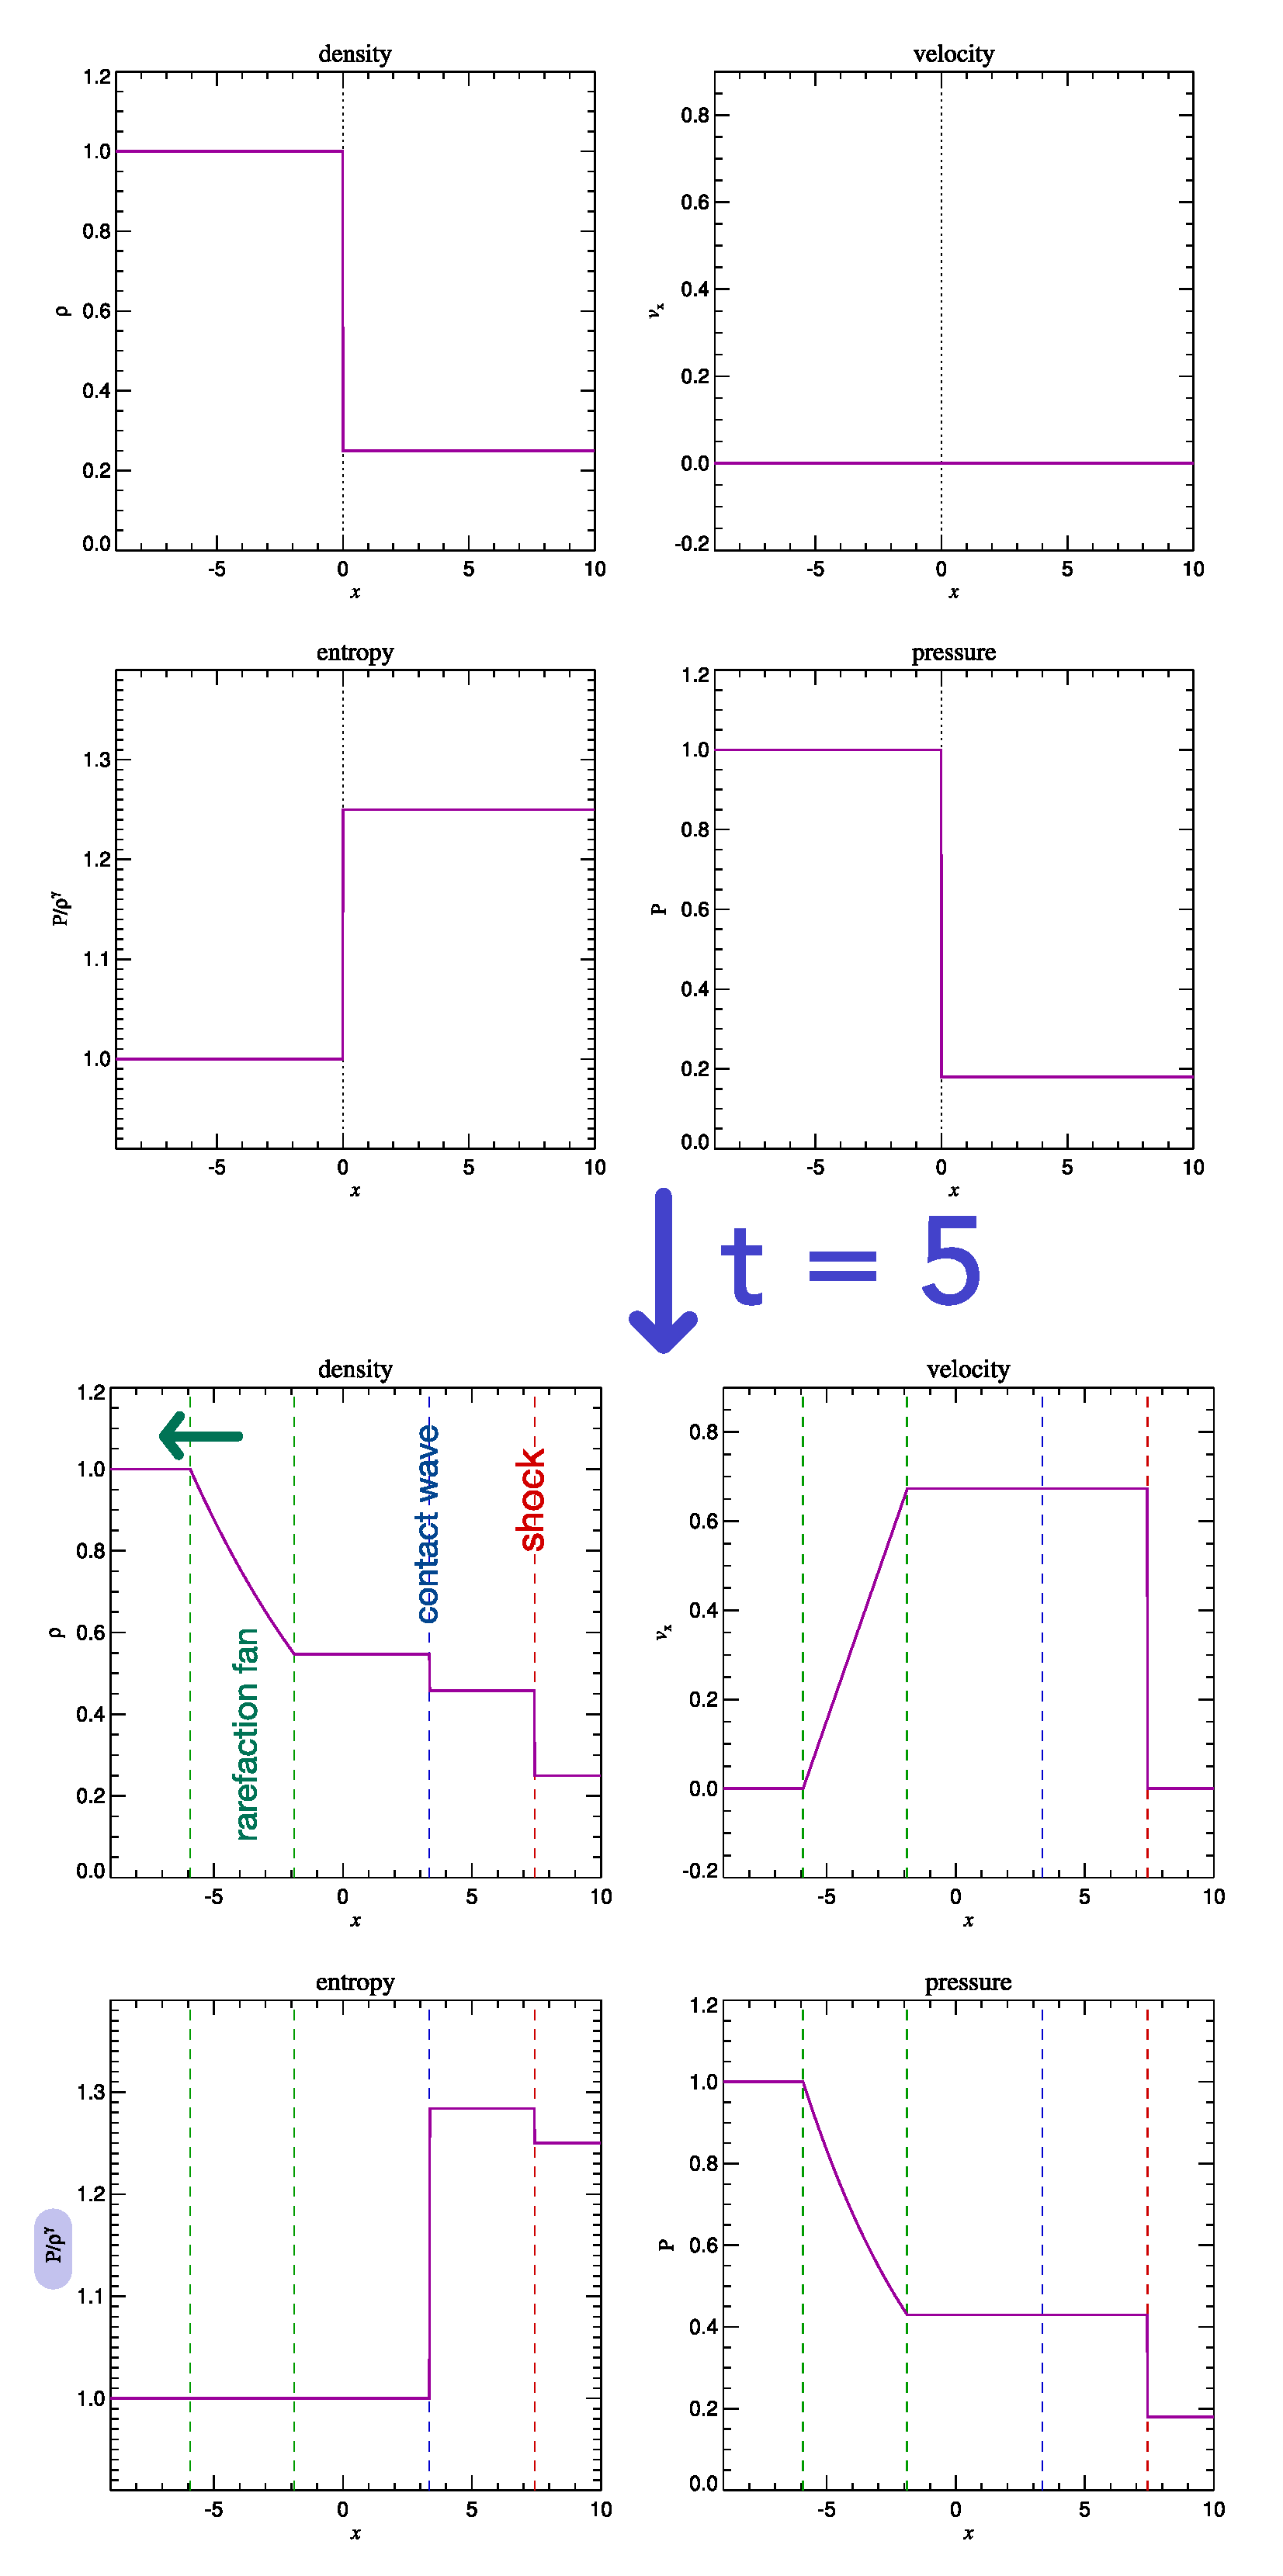
\includegraphics[width=0.6\textwidth]{figures/riemann_problem_example.pdf}
    \caption{Example Riemann-Problem situation}
    \label{fig:riemann_problem_example}
\end{figure}

\note{For an isentropic process $dS = 0$, the entropic function $A(s) = \frac{P}{\rho^\gamma} = \text{const.}$ so we can
use it as a proxy for entropy.}

\subsubsubsection{Properties of shock, contact discontinuity and rarefaction wave}
\begin{itemize}
    \item \textcolor{blue1}{Shock:} Normal velocity, pressure, denseity, entropy change discontinuously. In the rest frame of the shock fast upstream fluid is converted to slow downstream one. The fluid is compressed and kinetic energy tuned into heat (addition of entropy).
    \item \textcolor{blue1}{Contact discontinuity:} Traces the original seperating plane between the two originally seperated fluid phases.
    \begin{itemize}
        \item \textcolor{blue1}{constant across the contact:} pressure, normal velocity
        \item \textcolor{blue1}{can jump:} density, entropy, temperature
    \end{itemize}
    \item \textcolor{blue1}{Rarefaction wave:} smooth transition between two states, no discontinuities
\end{itemize}

\subsection{Finite volume discretization | Reducing a hyperbolic conservation law to a Riemann problem | Godunov scheme}
\idea{If we discretize the fluid into finite volumes and assume constant fluid variables on them, at each cell interface we have a Riemann problem. We are now more concerned with cell boundaries than centers. In the - conservative, finite volume - Godunov method, exact or approximate Riemann problems are solved at the boundaries and no flux is lost.}

\subsubsection{Problem | solve a hyperbolic conservation law PDE}
We want to solve the conservation law
\begin{equation}
    \partial_t \vec{U} + \partial_\vec{x} \cdot \mat{F}(\vec{U}) = 0, \quad \text{state vector } \vec{U}, \quad \text{flux matrix } \mat{F}
\end{equation}
for instance for the Euler equations with
\begin{equation}
    \label{eq:euler_equations_vec}
    \vec{U} = \begin{pmatrix} \rho \\ \rho \vec{v} \\ \rho e \end{pmatrix}, \quad \mat{F} = \begin{pmatrix} \rho \vec{v} \\ \rho \vec{v} \vec{v}^T + P \mat{1} \\ (\rho e + P) \vec{v} \end{pmatrix}, \quad e = e_{th} + \frac{\vec{v}^2}{2}, \quad P = (\gamma - 1) \rho e_{th} \text{ closure}
\end{equation}

\subsubsection{Deriving a finite volume scheme where only Riemann problems are left to solve}
In a finite volume method, the state of the cell is an average over the fluid quantities over the cell
\begin{equation}
    \label{eq:cell_avg}
    \vec{U}_i = \frac{1}{V_i} \int_{\text{cell} i}{\vec{U}(\vec{x})} dV
\end{equation}
\greenbox{\textbf{Aim:} We want to derive an update scheme for the cell averages $\vec{U}_i$ (the vector of the fluid variables), where no intercell flux is lost.}
We derive the update scheme in 1D, so $\vec{F}$ is a vector ($\vec{v}\vec{v}^T$ is a scalar) (see figure \ref{fig:finite_volume_scheme}).

\begin{figure}[htb!]
    \centering
    \includesvg[width=0.8\textwidth]{figures/finite_volume_scheme2.svg}
    \caption{Finite volume scheme}
    \label{fig:finite_volume_scheme}
\end{figure}

\textcolor{blue1}{Step 1}: Integrate the conservation law over a cell and timestep and recognize the average
defined in \ref{eq:cell_avg}.

\begin{equation}
    \begin{gathered}
        \int_{x_{i-\frac{1}{2}}}^{x_{i+\frac{1}{2}}} \int_{t_n}^{t_{n+1}}\left(\frac{\partial \vec{U}}{\partial t}+\frac{\partial \vec{F}}{\partial x}\right) d t d x=0 \\
        \underbrace{=}_{\text{carry out simple integrals}} \int_{x_{i-\frac{1}{2}}}^{x_{i+\frac{1}{2}}}\left[\vec{U}\left(x, t_{n+1}\right)-\vec{U}\left(x, t_n\right)\right] d x+\int_{t_n}^{t_{n+1}}\left[\vec{F}\left(x_{i+\frac{1}{2}}, t\right)-\vec{F}\left(x_{i-\frac{1}{2}}, t\right)\right] dt \\
        \underbrace{=}_{\text{recognize avg}} \Delta x\left[\vec{U}_i^{(n+1)}-\vec{U}_i^{(n)}\right]+\int_{t_n}^{t_{n+1}}\left[\vec{F}\left(x_{i+\frac{1}{2}}, t\right)-\vec{F}\left(x_{i-\frac{1}{2}}, t\right)\right] d t=0
    \end{gathered}
    \label{eq:finite_volume_scheme_step1}
\end{equation}

\textcolor{blue1}{Step 2}: In the frame of discrete cell averages, \textcolor{blue1}{between any two cells we essentially have a Riemann problem from which solution we can follow the flux between the cells}.
\begin{equation}
    \vec{F}(x_{i+\frac{1}{2}},t) \text{ for } t > t_n = \text{solution of Riemann problem with left state } \vec{U}_i^{(n)} \text{ and right state } \vec{U}_{i+1}^{(n)}
\end{equation}
\note{At the cell interface, the solution of the Riemann problem is constant in time, so
\begin{equation}
    \vec{F}(x_{i+\frac{1}{2}},t) = \vec{F}^*_{i+\frac{1}{2}} = \vec{F}_{\text{Riemann}}(\vec{U}_i^{(n)}, \vec{U}_{i+1}^{(n)}) \text{ from Riemann solution at interface }
\end{equation}
}
\begin{mdframed}[style=padded]
    \textcolor{blue1}{Step 3}: As the solution at the interface is constant, without approximation, we can write the \textcolor{blue1}{Godunov scheme} (based on eq. \ref{eq:finite_volume_scheme_step1}) as
    \begin{equation}
        \vec{U}_i^{(n+1)}=\vec{U}_i^{(n)}+\frac{\Delta t}{\Delta x}\left[\underbrace{\vec{F}^*_{i-\frac{1}{2}}}_{\text{flux from left into cell}}-\underbrace{\vec{F}^*_{i+\frac{1}{2}}}_{\text{out on the right}}\right]
    \end{equation}
    This defines an update scheme for the fluid variables on the cells (with some appropriate initial and boundary conditions). $\vec{F}^*_{i-\frac{1}{2}}$ and $\vec{F}^*_{i+\frac{1}{2}}$ are black-boxes for now - to find the fluxes we need to solve the Riemann problem, later e.g. done with the approximate HLL solver.
\end{mdframed}

\subsubsubsection{Caveats of the Godunov scheme}
\textcolor{red1}{CFL needs to be obeyed:} We can only assume the Riemann problems at the interfaces to be independent, if the timestep is short enough, so that no information has travelled from one interface to the other $\rightarrow$ CFL: $\frac{\Delta x}{\Delta t} \geq c_{max}$.

\textcolor{red1}{$\vec{U}$ is not piecewise constant in reality:} Even if we start out with piecewise constant $\vec{U}$ in reality, this will change. Therefore the flux we calculate between the cells is also only an approximation.

\subsubsection{Godunov's method and Riemann solver | reconstruct - evolve - average (REA)}
Godunov's method can be seen as a REA scheme of a hydrodynamical system discretized on a mesh
\begin{enumerate}
    \item \textcolor{blue1}{Reconstruct:} A global solution is constructed from the cell averaged quantities, simples approach: piecewise-constant
    \item \textcolor{blue1}{Evolve:} The reconstructed state is evolved by $\Delta t$ (mind the CFL criterion), in the Gudonov scheme based on the intercell Riemann problems
    \item \textcolor{blue1}{Average:} $\vec{U}_i^{(n+1)}$ is calculatted from the evolved state, in the Godunov scheme, evolving and averaging are combined as we directly calculate the new average based on accounting the fluxes entering and leaving the cell (an implicit average over the new state)
\end{enumerate}

\yellowbox{But how can the Riemann problem giving us the fluxes be solved?}

\subsection{Approximate Riemann solvers | HLL solver}
\subsubsection{1D Riemann problem to solve}
Let us again formulate the Riemann problem in 1D.
Given the conservation law
\begin{equation}
    \partial_t u(x) + \partial_x f(u) = 0
\end{equation}
with piecewise initial values
\begin{equation}
    u(x, t=0)=\left\{\begin{array}{l}
    u_L \text { for } x<0 \\
    u_R \text { for } x \geq 0
    \end{array}, \quad \text { cell interface at } x=0\right.
\end{equation}
we want to solve for our fluid quantity $u$. The characteristics,
i.e. where information from point $x = 0$ (discontinuity) can travel
in some time, are shown in figure \ref{fig:char_hll}.

\begin{figure}[htb!]
    \centering
    \includesvg[width=0.8\textwidth]{figures/hll2.svg}
    \caption{Characteristics of the Riemann problem and HLL approach.}
    \label{fig:char_hll}
\end{figure}

\subsubsection{Basic HLL assumptions and problem statement}
In the HLL scheme we assume to know
\begin{itemize}
    \item the fastest moving wave velocity to the left $S_L$ and right $S_R$
    \item the left and right state $u_L$ and $u_R$ and therefore the fluxes $f_L$ and $f_R$
\end{itemize}
Based on the CFL criterion (no interaction with other cells), we can assume the following quantities to be constant in time $t \in [0, T]$:
\begin{equation}
    u_L = u(x_L, t), \quad u_R = u(x_R, t), \quad f_L = f(u_L), \quad f_R = f(u_R)
\end{equation}
and we make the simplifying assumption that
\begin{equation}
    \forall x \in [S_R t, S_L t]: u(x, t) = u^{HLL} = u_L^* = u_R^* = u^* \underbrace{=}_{\text{at interface}} \text{const.}, \quad f^{HLL} = f^* = f_L^* = f_R^*
\end{equation}
\greenbox{\textbf{Aim:} Find expressions for $u^*$ and $f^*$.}

\subsubsection{Deriving the solution of the Riemann problem in the HLL scheme}
\idea{$u$ is conserved, so the spatial integral over $u$ at some point in time is the same as at another point in time
plus / minus the in- and outcoming fluxes during that time-interval. Based and the flux balance in our whole
region $[x_L, x_R]$ we can first find an expression for $u^{HLL}$ and then based on the same balance in
the left and right region $[S_R T, 0]$ and $[0, S_L T]$ we can find an expression for $f^{HLL}$.}

\subsubsubsection{Derivation of the middle state $u^{HLL}$ at $t = T$}
Remember, we assume the middle state $u^{HLL}$ hold for the whole interval $[S_R T, S_L T]$, where
information could have spread.

We can therefore write
\begin{equation}
    u^{HLL} = \frac{1}{T\cdot(S_R - S_L)} \mathcolor{red1}{\int_{TS_R}^{TS_L}{u(x,T)}dx}
\end{equation}
we can find \textcolor{red1}{this} integral from considering the spatial
integral over the whole domain at time $T$
\begin{equation}
    \begin{aligned}
        \int_{x_L}^{x_R} u(x, T) d x&=\left(T S_L-x_L\right) u_L+\mathcolor{red1}{\int_{T S_R}^{T S_L} u(x, T) dx}+\left(x_R-T S_R\right) u_R \\
                                    &{\underbrace{=}_{u \text{ conserved}}} \mathcolor{green1}{\int_{x_L}^{x_R} u(x, 0) d x}+\underbrace{\int_0^T f\left(u_L\right) d t}_{\text{flux in from left}}-\underbrace{\int_0^T f\left(u_R\right) d t}_{\text{flux out to right}} \\
                                    &= \mathcolor{green1}{u_R x_R - u_L x_L} + f_L T - f_R T
    \end{aligned}
\end{equation}
We therefore find an expression for \textcolor{red1}{our integral} and thus for $u^{HLL}$:
\begin{equation}
    u^{H L L}=\frac{S_R u_R-S_L u_L+f_L-f_R}{S_R-S_L}
\end{equation}
Which is a pretty simple balance we could have seen directly, by
\begin{equation}
    \text{start state} \cdot \text{volume} + \text{net flux into volume} \cdot \Delta t = \text{end state} \cdot \text{volume}
\end{equation}
over $[\Delta t S_L,\Delta t S_R]$.

\subsubsubsection{Deriving the intercell flux $f^{HLL} = f^*$}
We consider the integral over $u$ in the left region where the
information can have propagated to, so $x \in [S_R T, 0]$ and
in the right region $x \in [0, S_L T]$.
\idea{As before the integral of $u$ over space at some time $t$ must be the same as at an earlier time plus / minus the fluxes in / out since then.}
For the left ($x \in [S_L T, 0]$) we have
\begin{equation}
    \begin{aligned}
        -T S_L u^{H L L}= & \int_{T S_L}^0 u(x, T) d x \\
        & = \underbrace{-T S_L u_L}_{\text{at t} = 0} + \underbrace{T \cdot\left(f_L-f_L^*\right)}_{\text{fluxes since then}}
    \end{aligned}
\end{equation}

For the right ($x \in [0, S_R T]$) we have
\begin{equation}
    \begin{aligned}
        T S_R u^{H L L}= & \int_{0}^{T S_R} u(x, T) d x \\
        & = \underbrace{T S_R u_R}_{\text{at t} = 0} + \underbrace{T \cdot\left(f_R^*-f_R\right)}_{\text{fluxes since then}}
    \end{aligned}
\end{equation}

The fluxes at the interface must be equal, $f_L^* = f_R^* = f^{HLL}$, so
\begin{equation}
    f^{H L L}=f_L+S_L\left(u^{H L L}-u_L\right)=f_R+S_R\left(u^{H L L}-u_R\right)
\end{equation}

\subsubsection{Final HLL solution}
There are three states after the step $T$ in the HLL scheme
\begin{equation}
    u(x, T)=\left\{\begin{array}{c}
    u_L \text { for } x<S_L t \\
    u^{H L L} \text { for } S_L t \leq x \leq S_R t \\
    u_R \text { for } x>S_R t
    \end{array}\right.
\end{equation}
and the interface flux is
\begin{equation}
    \begin{gathered}
        f^{H L L}=\frac{S_R f_R-S_L f_L+S_L S_R\left(u_R-u_L\right)}{S_R-S_L} \\
        \text{maximum velocity to the left } S_L, \quad \text{maximum velocity to the right } S_R \\
        \text{initial state on the left } u_L, \quad \text{initial state on the right } u_R \\
        f_L = f(u_L), \quad f_R = f(u_R)
    \end{gathered}
\end{equation}

\subsubsection{Mind that the extreme velocities can point into the same direction}
Both extreme velocities can be to the left, both to the right, or on to the left and one to the right.
For instance in figure \ref{fig:adv_char} characteristics for advection are drawn.

\begin{figure}[htb!]
    \centering
    \includesvg[width=0.8\textwidth]{figures/adv_char.svg}
    \caption{Advection characteristics, once the simple advection case with only the advection speed and once with information travelling from the advected state to the left and right with the speed of sound.}
    \label{fig:adv_char}
\end{figure}

\subsubsection{Godunov scheme with HLL solver}
For the Godunov scheme
\begin{equation}
    U_i^{(n+1)} = U_i^{(n)} + \frac{\Delta t}{\Delta x} \left[ F^*_{i-\frac{1}{2}} - F^*_{i+\frac{1}{2}} \right]
\end{equation}
the flux we choose depends on the orientation of $S_L$ and $S_R$ (eveloping the \textit{Lichtkegel}).
This is illustrated for unidirectional information flow to the right in figure \ref{fig:godunov_unidir}.

\begin{figure}[htb!]
    \centering
    \includesvg[width=0.8\textwidth]{figures/unidirectional_inf.svg}
    \caption{Godunov scheme with HLL solver for unidirectional information flow to the right.}
    \label{fig:godunov_unidir}
\end{figure}

We get
\begin{equation}
    F_{i+\frac{1}{2}}^*=\left\{\begin{array}{c}
        F_i \text { for } 0<S_L \\
        F_{i+\frac{1}{2}}^{H L L} \text { for } S_L \leq 0 \leq S_R\\
        F_{i+1} \text { for } 0>S_R
        \end{array}\right., \quad F_{i-\frac{1}{2}}^* \text { from } i \rightarrow i-1 
\end{equation}
with
\begin{equation}
    F_{i+\frac{1}{2}}^{H L L}=\frac{S_R F_{i+1}-S_L F_i+S_L S_R\left(U_{i+1}-U_i\right)}{S_R-S_L}
\end{equation}
where we can combine this expression and the cases above to
\begin{equation}
    F_{i+\frac{1}{2}}^{H L L}=\frac{S_R^+ F_{i+1}-S_L^- F_i+S_L^- S_R^+\left(U_{i+1}-U_i\right)}{S_R^+-S_L^-}, \quad S_R^+ = \max(0, S_R), \quad S_L^- = \min(0, S_L)
\end{equation}

\subsubsection{Pointers to extensions of the HLL scheme}
\begin{itemize}
    \item in HLLC an additional velocity between $S_L$ and $S_R$ is considered
    \item HLLD used for magnetohydrodynamics (MHD)
\end{itemize}

\subsubsection{Ansätze for the maximum wave velocities $S_L$ and $S_R$}
Consider the gas velocity $v$ as given by part of the state vector and
sound speed $c_s$ (depending on the state on each side, e.g. $c_s^2 = \gamma P \slash \rho$ for
and adiabatic process, here called $a_L$ and $a_R$), then
possible estimates are
\begin{itemize}
    \item $S_L = v_L - a_L, S_R = v_R + a_R$
    \item $S_L = \min(v_L - a_L, v_R - a_R), S_R = \max(v_R + a_R, v_R + a_R)$
    \item Roe average, where we weigh dense areas as more important to the communication (leading to less smearing but \textcolor{red1}{instability})
          of information.
          \begin{equation}
            \begin{aligned}
            S_L & =\tilde{u}-\tilde{a} \\
            S_R & =\tilde{u}+\tilde{a} \\
            \tilde{u} & =\frac{\sqrt{\rho_L} u_L+\sqrt{\rho_R} u_R}{\sqrt{\rho_L}+\sqrt{\rho_R}} \\
            \tilde{a} & =\left[(\gamma-1)\left(\widetilde{H}-\frac{1}{2} \tilde{u}^2\right)\right]^{\frac{1}{2}} \text { with the enthalpy } \\
            H & =(e+P) / \rho \text { and } \\
            \widetilde{H} & =\frac{\sqrt{\rho_L} H_L+\sqrt{\rho_R} H_R}{\sqrt{\rho_L}+\sqrt{\rho_R}}
            \end{aligned}
        \end{equation}
\end{itemize}

\subsection{Extension of Eulerian hydrodynamics to multiple dimensions}
Based on our previous results, we can simulate the 1D conservation law
\begin{equation}
    \partial_t \vec{U} + \partial_x \vec{F}(\vec{U}) = 0
\end{equation}
e.g. for an isothermal gas (so constant sound speed $c_s$) with
\begin{equation}
    \vec{U} = \begin{pmatrix} \rho \\ \rho v_x \end{pmatrix}, \quad \vec{F} = \begin{pmatrix} \rho v_x \\ \rho v_x^2 + P \end{pmatrix}, \quad P = c_s^2 \rho
\end{equation}
Let us formulate the \textcolor{blue1}{Euler equations for a 3D fluid} (see eq. \ref{eq:euler_equations_vec}) by seperating the flux by direction
\begin{equation}
    \label{eq:3d_split}
    \partial_t \vec{U} + \partial_x \vec{F} + \partial_y \vec{G} + \partial_z \vec{H} = 0
\end{equation}
with
\begin{equation}
    \begin{gathered}
        \vec{F}: \text{ flux vector along } \vec{\hat{e}}_x, \quad \vec{G}: \text{ flux vector along } \vec{\hat{e}}_y, \quad \vec{H}: \text{ flux vector along } \vec{\hat{e}}_z \\
        \vec{F}=\left(\begin{array}{c}
            \rho u \\
            \rho u^2+P \\
            \rho u v \\
            \rho u w \\
            u(\rho e+P)
            \end{array}\right), \quad \vec{G}=\left(\begin{array}{c}
            \rho v \\
            p u v \\
            \rho v^2+P \\
            \rho v w \\
            v(\rho e+P)
            \end{array}\right), \quad \vec{U}=\left(\begin{array}{c}
            \rho w \\
            p u w \\
            \rho v w \\
            \rho w^2+P \\
            w(\rho e+P)
            \end{array}\right) \\
        \text{state vector } \vec{U} = \left(\begin{array}{c}
            \rho \\
            \rho u \\
            \rho v \\
            \rho w \\
            \rho e
            \end{array}\right)
    \end{gathered}
\end{equation}
and
\begin{equation}
    \begin{gathered}
        \text{total specific energy per uni mass } e = e_{th} + \frac{1}{2} \left( u^2 + v^2 + w^2 \right) \\
        \text{pressure } P = (\gamma - 1) \rho e_{th}, \quad \text{thermal energy per unit mass } e_{th} \\
        u: \text{ velocity in } \vec{\hat{e}}_x \text{ direction}, \quad v: \text{ velocity in } \vec{\hat{e}}_y \text{ direction}, \quad w: \text{ velocity in } \vec{\hat{e}}_z \text{ direction}
    \end{gathered}
\end{equation}

\subsubsection{Dimensional splitting Ansatz}
\idea{Seperately update dimensions (using our 1D solver) and combine.}
From eq. \ref{eq:3d_split} we make the following separation ansatz
\begin{equation}
    \partial_t \vec{U} + \partial_x \vec{F} = \vec{0}, \quad \partial_t \vec{U} + \partial_y \vec{G} = \vec{0}, \quad \partial_t \vec{U} + \partial_z \vec{H} = \vec{0}
\end{equation}
\note{While the state vector and fluxes are still $\in \mathbb{R}^5$ (the velocities in the other directions appear), we effectively have \textit{augmented} 1D problems (the flux along $x$ is not as directly coupled to $w$ as it is to $u$)}
To forward our state in 3D we have to sequence multiple augmented 1D steps (sweeps). For 2D this
is illustrated in figure \ref{fig:2d_sweep}.

\begin{figure}[htb!]
    \centering
    \includesvg[width=0.9\textwidth]{figures/2dsplitting.svg}
    \caption{Splitting Ansatz for 2D}
    \label{fig:2d_sweep}
\end{figure}

\subsubsubsection{1st order ansatz}
Assuming we already have a method to advance in one dimension then
\begin{equation}
    \vec{U}^{(n+1)} = \mathcal{X}(\Delta t) \mathcal{Y}(\Delta t) \mathcal{Z}(\Delta t) \vec{U}^{(n)}, \quad \text{time evolution operators} \mathcal{X}, \mathcal{Y}, \mathcal{Z}
\end{equation}
is a dimensionally split update scheme, which is exact for linear advection but
not so for any higher order problem (first order reduction) as the steps
in the dimensions are done separately.

\subsubsubsection{2nd order accurate in 2D examples}
\begin{equation}
    \begin{gathered}
    \vec{U}^{(n+1)}=\frac{1}{2}[\mathcal{X}(\Delta t) \mathcal{Y}(\Delta t)+\mathcal{Y}(\Delta t) \mathcal{X}(\Delta t)] \vec{U}^{(n)} \\
    \text { or } \vec{U}^{(n+1)}=\mathcal{X}\left(\frac{\Delta t}{2}\right) \mathcal{Y}(\Delta t) \mathcal{X}\left(\frac{\Delta t}{2}\right) \vec{U}^{(n)}
    \end{gathered}
\end{equation}

\subsubsection{2nd order accurate in 3D example}
\begin{equation}
    \vec{U}^{(n+1)}=\mathcal{X}\left(\frac{\Delta t}{2}\right) \mathcal{Y}\left(\frac{\Delta t}{2}\right) \mathcal{Z}(\Delta t) \mathcal{Y}\left(\frac{\Delta t}{2}\right) \mathcal{X}\left(\frac{\Delta t}{2}\right) \vec{U}^{(n)}
\end{equation}
where the 2nd order is based on the alternating reverse order application of
the time evolution operators.

\subsubsection{Unsplit schemes}
Consider rectangular 2D cells. In a dimensionally split scheme we would 
make updates to a cell based on the information flow in only one direction 
and then the other based on the changed situation. In an unsplit scheme we 
apply both fluxes simultaneously.

In the case of rectangular cells in 2D, we have
\begin{equation}
    \vec{U}_{i, j}^{(n+1)}=\vec{U}_{i, j}^{(n)}+\frac{\Delta t}{\Delta x}\left(\vec{F}_{i-\frac{1}{2}, j}-\vec{F}_{i+\frac{1}{2}, j}\right)+\frac{\Delta t}{\Delta y}\left(\vec{G}_{i, j-\frac{1}{2}}-\vec{G}_{i, j-\frac{1}{2}}\right)
\end{equation}
\todo[inline]{Shouldn't this be all fluxes divided by the area of the cell?}

In the situation of an unstructured mesh, we generally have
\begin{equation}
    \begin{gathered}
        \vec{U}^{(n+1)}=\vec{U}^{(n)}-\frac{\Delta t}{V} \int \vec{F} \cdot d \vec{S} \text { integral over cell surface} \\
        d\vec{S} \text{ is the surface element vector, pointing outwards}
    \end{gathered}
\end{equation}
which makes sense intuitively (the change coming from the
borders distributes over the cells).

The situations are illustrated in figure \ref{fig:usplit}.
\begin{figure}[htb!]
    \centering
    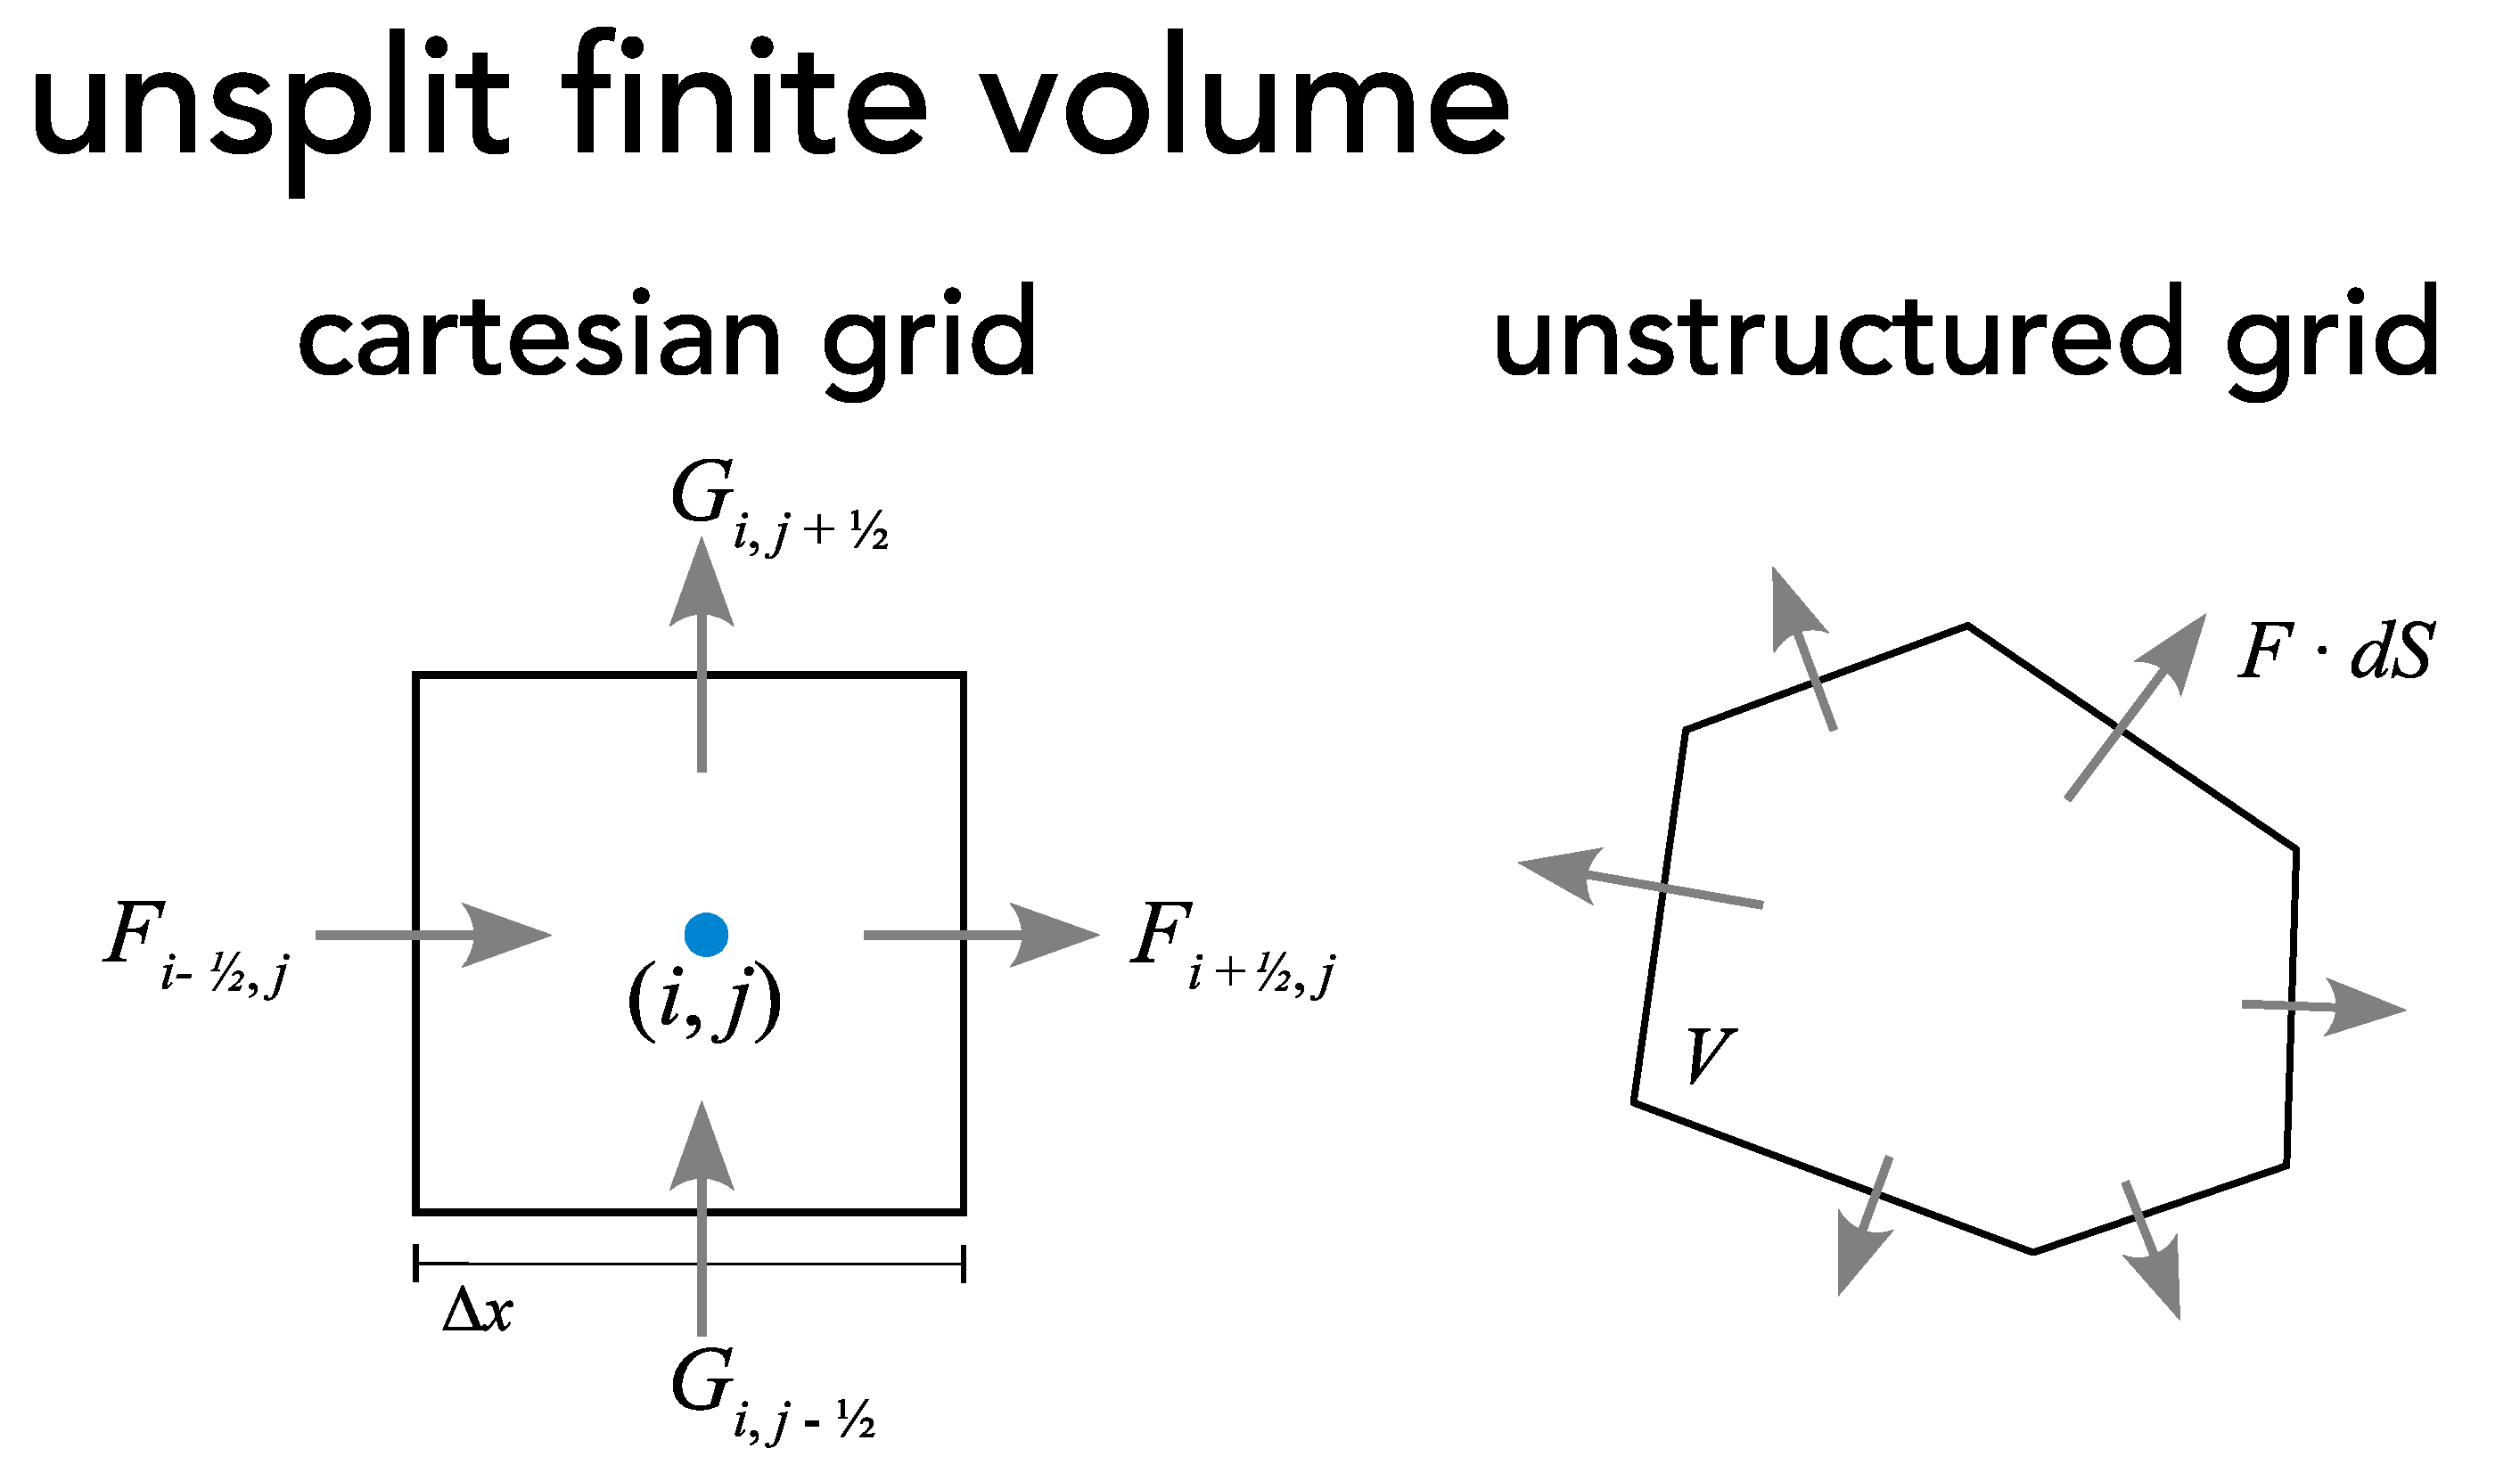
\includegraphics[width=0.9\textwidth]{figures/usplit.pdf}
    \caption{Unsplitting Ansatz Grids}
    \label{fig:usplit}
\end{figure}

\subsection{Extensions for high-oder accuracy}
\subsubsection{What even is a schemes order?}
Consider our numerical solution $\rho_i$ sits on a grid of $N$ points $x_i$, $i = 1, \dots, N$.
Let $\rho(x)$ be the true solution. Then based on the mean L1 error
\begin{equation}
    L1 = \frac{1}{N} \sum_{i=1}^{N}{\left| \rho_i - \rho(x_i) \right|}
\end{equation}
we call a method
\begin{itemize}
    \item \textcolor{blue1}{first order accurate} if $L1 \propto \Delta x \propto N^{-1}$ with $\Delta x = \frac{L}{N}$
    \item \textcolor{blue1}{second order accurate} if $L1 \propto \Delta x^2 \propto N^{-2}$
    \item ...
\end{itemize}
In the 2nd order accurate scheme, doubling the number of cells will quarter our error.

\subsubsection{2nd order extension to Godunov's scheme by changing the reconstruction step from piecewise-constant to linear}

\bluebox{\textbf{Godunov's theorem states:} Linear numerical 
schemes for solving partial differential equations (PDE's), 
having the property of not generating new extrema (monotone 
scheme), can be at most first-order accurate\footnote{In Godunov's scheme the dissipation is
just strong enough to damp shorter waves before they get too much out of step and
show up as oscillations on top of the larger features.}. Bram van Leer (and Vladimir P. Kolgan\footnote{Already in 1972, he developed a scheme 2nd order in space (using the (\textit{crude}) minmod limiter) but only first order in time, using Forward Euler. Sadly, he succumbed to lung cancer in 1978, at the
age of 37.})
first succeeded in \textbf{circumventing this} by nolinearly limiting the second order
term as a function of the non-smoothness of the numerical solution (sustaining monotonicity)
(a non-linear technique even for a linear equation, see flux limiters later on)
(so we have (at least) 2nd order accuracy where the flow is smooth) (e.g. \cite{leer79}).}

\begin{enumerate}
    \item Estimate the fluid variables gradients, e.g. $\partial_x\rho$ (e.g. based on the averages on the neighboring cells)
    \item Slope limit these gradients as otherwise we could introduce quite extreme values of the fluid variables at the cell boundaries, especially in case real fluid discontinuities are present
    \item Estimate the values of the fluid variables at one interface by linear extrapolation
    \begin{equation}
        \mathcolor{red1}{\rho_{i+\frac{1}{2}}^L = \rho_i + \frac{\Delta x}{2} (\partial_x \rho)_i}, \quad \mathcolor{red1}{\rho_{i+\frac{1}{2}}^R = \rho_{i+1} - \frac{\Delta x}{2} (\partial_x \rho)_{i+1}}
    \end{equation}
    See figure \ref{fig:linear_extrapolation} for an illustration.
    \begin{figure}[htb!]
        \centering
        \includesvg[width=0.8\textwidth]{figures/1dreconst.svg}
        \caption{Linear extrapolation of the fluid variables to the cell interface.}
        \label{fig:linear_extrapolation}
    \end{figure}
    \item Based on the extrapolated fluid variable values at the interface we apply our Riemann solver to find the flux and update the cell averages (although we do not have the piecewise-constant Riemann situation)
\end{enumerate}

\problem{Above we have done a linear extrapolation to the boundary $\rho_{i+\frac{1}{2}}^L$ based on the gradient at the center $(\partial_x \rho)_i$. Note, however, that over our timestep
$\Delta t$, $\rho_i$ changes, so also our value at the boundary.
\begin{equation}
    d\rho(x,t) = (\partial_x \rho) dx + (\partial_t \rho) dt
\end{equation}
}
For more stability (and 2nd order accuracy), we do the extrapolation based on the gradient but also include the effect of $(\partial_t \rho)_i$ up intil half a timestep (as a proxy to the situation throughout the timestep).
\begin{equation}
    \begin{gathered}
        \rho_{i+\frac{1}{2}}^L=\rho_i+\left(\partial_x \rho\right)_i \frac{\Delta x}{2}+\left(\partial_t \rho\right)_i \frac{\Delta t}{2}, \quad \rho_{i+\frac{1}{2}}^R=\rho_{i+1}-\left(\partial_x \rho\right)_{i+1} \frac{\Delta x}{2}+\left(\partial_t \rho\right)_{i+1} \frac{\Delta t}{2} \\
        \rightarrow \text{ flux estimate } \vec{F}_{\text{Riemann}}\left( \vec{U}_{i+\frac{1}{2}}^L, \vec{U}_{i+\frac{1}{2}}^R \right) \text{ effectively at half-timestep}
    \end{gathered}
\end{equation}
So for the entire state $\vec{U}$ we have
\begin{equation}
    \begin{gathered}
        \vec{U}_{i+\frac{1}{2}}^L=\vec{U}_i+\mathcolor{yellow1}{\left(\partial_x \vec{U}\right)_i} \frac{\Delta x}{2}+\mathcolor{blue1}{\left(\partial_t \vec{U}\right)_i} \frac{\Delta t}{2}, \quad \vec{U}_{i+\frac{1}{2}}^R=\vec{U}_{i+1}-\mathcolor{yellow1}{\left(\partial_x \vec{U}\right)_{i+1}}  \frac{\Delta x}{2}+ \mathcolor{blue1}{\left(\partial_t \vec{U}\right)_{i+1}} \frac{\Delta t}{2} \\
        \mathcolor{yellow1}{\left(\partial_x \vec{U}\right)_i \text{ calculated from finite difference approach + slope limiting}}
    \end{gathered}   
\end{equation}

\greenbox{\textbf{Idea of the MUSCL-Hancock scheme:} Cell averages of the primitive fluid quantities are used to predict the values at the cell boundaries as $t + \frac{\Delta t}{2}$ and then use these prediction to calculate the fluxes and with them the primitive fluid quantities at $t + \Delta t$.}	

\subsubsubsection{How to estimate the \textcolor{blue1}{time derivatives $(\partial_t \vec{U})_i$}? | MUSCL-Hancock scheme}
Let us use the Euler equation in 1D ($x$ is a scalar)
\begin{equation}
    \begin{gathered}
        \partial_t \vec{U} + \partial_x \vec{F}(\vec{U}) \underbrace{=}_{\text{quasi-linear form}} \partial_t \vec{U} + \mat{J}_\vec{U}(\vec{F})\cdot \partial_x \vec{U} = 0 \rightarrow \boxed{\partial_t \vec{U} = - \mat{J}_\vec{u}(\vec{F})\cdot \partial_x \vec{U}} \\
        \text{with Jacobian matrix } \mat{J}_\vec{U}(\vec{F}) \text{ of } \vec{F}(\vec{U}) \text{ with respect to } \vec{U}, \quad \left. \mat{J}_\vec{U}(\vec{F}) \right|_{\vec{U} = \vec{U}} =: \mat{A}(\vec{U})
    \end{gathered}
\end{equation}
\begin{mdframed}[style=padded]
We can therefore estimate the derivative in time based on our estimation $\partial_x \vec{U}$ of the derivative in space, yielding
the \textcolor{blue1}{MUSCL-Hancock scheme} (Monotonic Upstream Scheme for Conservation Laws)
\begin{equation}
    \begin{aligned}
    & \vec{U}_{i+\frac{1}{2}}^L=\vec{U}_i+\left[\frac{\Delta x}{2} \underline{\underline{1}}-\mat{A}(\vec{U}) \frac{\Delta t}{2}\right]\mathcolor{yellow1}{\left(\partial_x \vec{U}\right)_{i}} \\
    & \\
    & \vec{U}_{i+\frac{1}{2}}^R=\vec{U}_{i+1}+\left[-\frac{\Delta x}{2} \mat{1}-\mat{A}(\vec{U}) \frac{\Delta t}{2}\right]\mathcolor{yellow1}{\left(\partial_x \vec{U}\right)_{i+1}}
    \end{aligned}
\end{equation}
- a 2nd order accurate extension of Godunov's scheme.
\end{mdframed}

\subsubsection{Idea and discussion of even higher order methods}
We can 
\begin{itemize}
    \item use higher order polynomial reconstruction as in piecewise parabolic methods (also mind information transport by characteristic waves), see figure \ref{fig:ppm} (high order methods tend to create post shock oscillations $\rightarrow$ add dissipation mechanism / some flattening\footnote{Which essentially means that locally we go back to lower order.} to PPM)
    \item even higher order polynomials are used in methods like ENO and WENO (find polynomials based on values from multiple cells (\textit{larger stencil}))
\end{itemize}

\begin{figure}[htb!]
    \centering
    \includesvg[width=0.8\textwidth]{figures/ppm.svg}
    \caption{Piecewise parabolic reconstruction.}
    \label{fig:ppm}
\end{figure}

\note{Independent of the order, we only \textbf{store} one value (per variable) per cell in finite volume methods. In \textbf{finite element methods}, per cell polynomial representations of the state vector are stored (discontinuities are harder to capture though).}

\subsubsubsection{Discussion of higher order methods}
Advantages and disadvantages of higher order methods can be found in table \ref{tab:high_order}, those
of lower order methods in table \ref{tab:low_order}.

\begin{table}[htb!]
    \centering
    \begin{tabular}{|p{0.45\textwidth}|p{0.45\textwidth}|}
        \hline
        \textcolor{green1}{Pro higher} & \textcolor{red1}{Con higher} \\
        \hline
        \begin{itemize}
            \item sharp solution
            \item more accurate (sharper solutions alone can be inaccurate, e.g. when the bulk position is inaccurate)
        \end{itemize}
        &
        \begin{itemize}
            \item more expensive
            \item strong oscillations at discontinuities (principle illustrated in figure \ref{fig:high_order_oscillations})
            \item crash at high Mach numbers
        \end{itemize} \\
        \hline
    \end{tabular}
    \caption{Advantages and disadvantages of higher order methods.}
    \label{tab:high_order}
\end{table}

\begin{figure}[htb!]
    \centering
    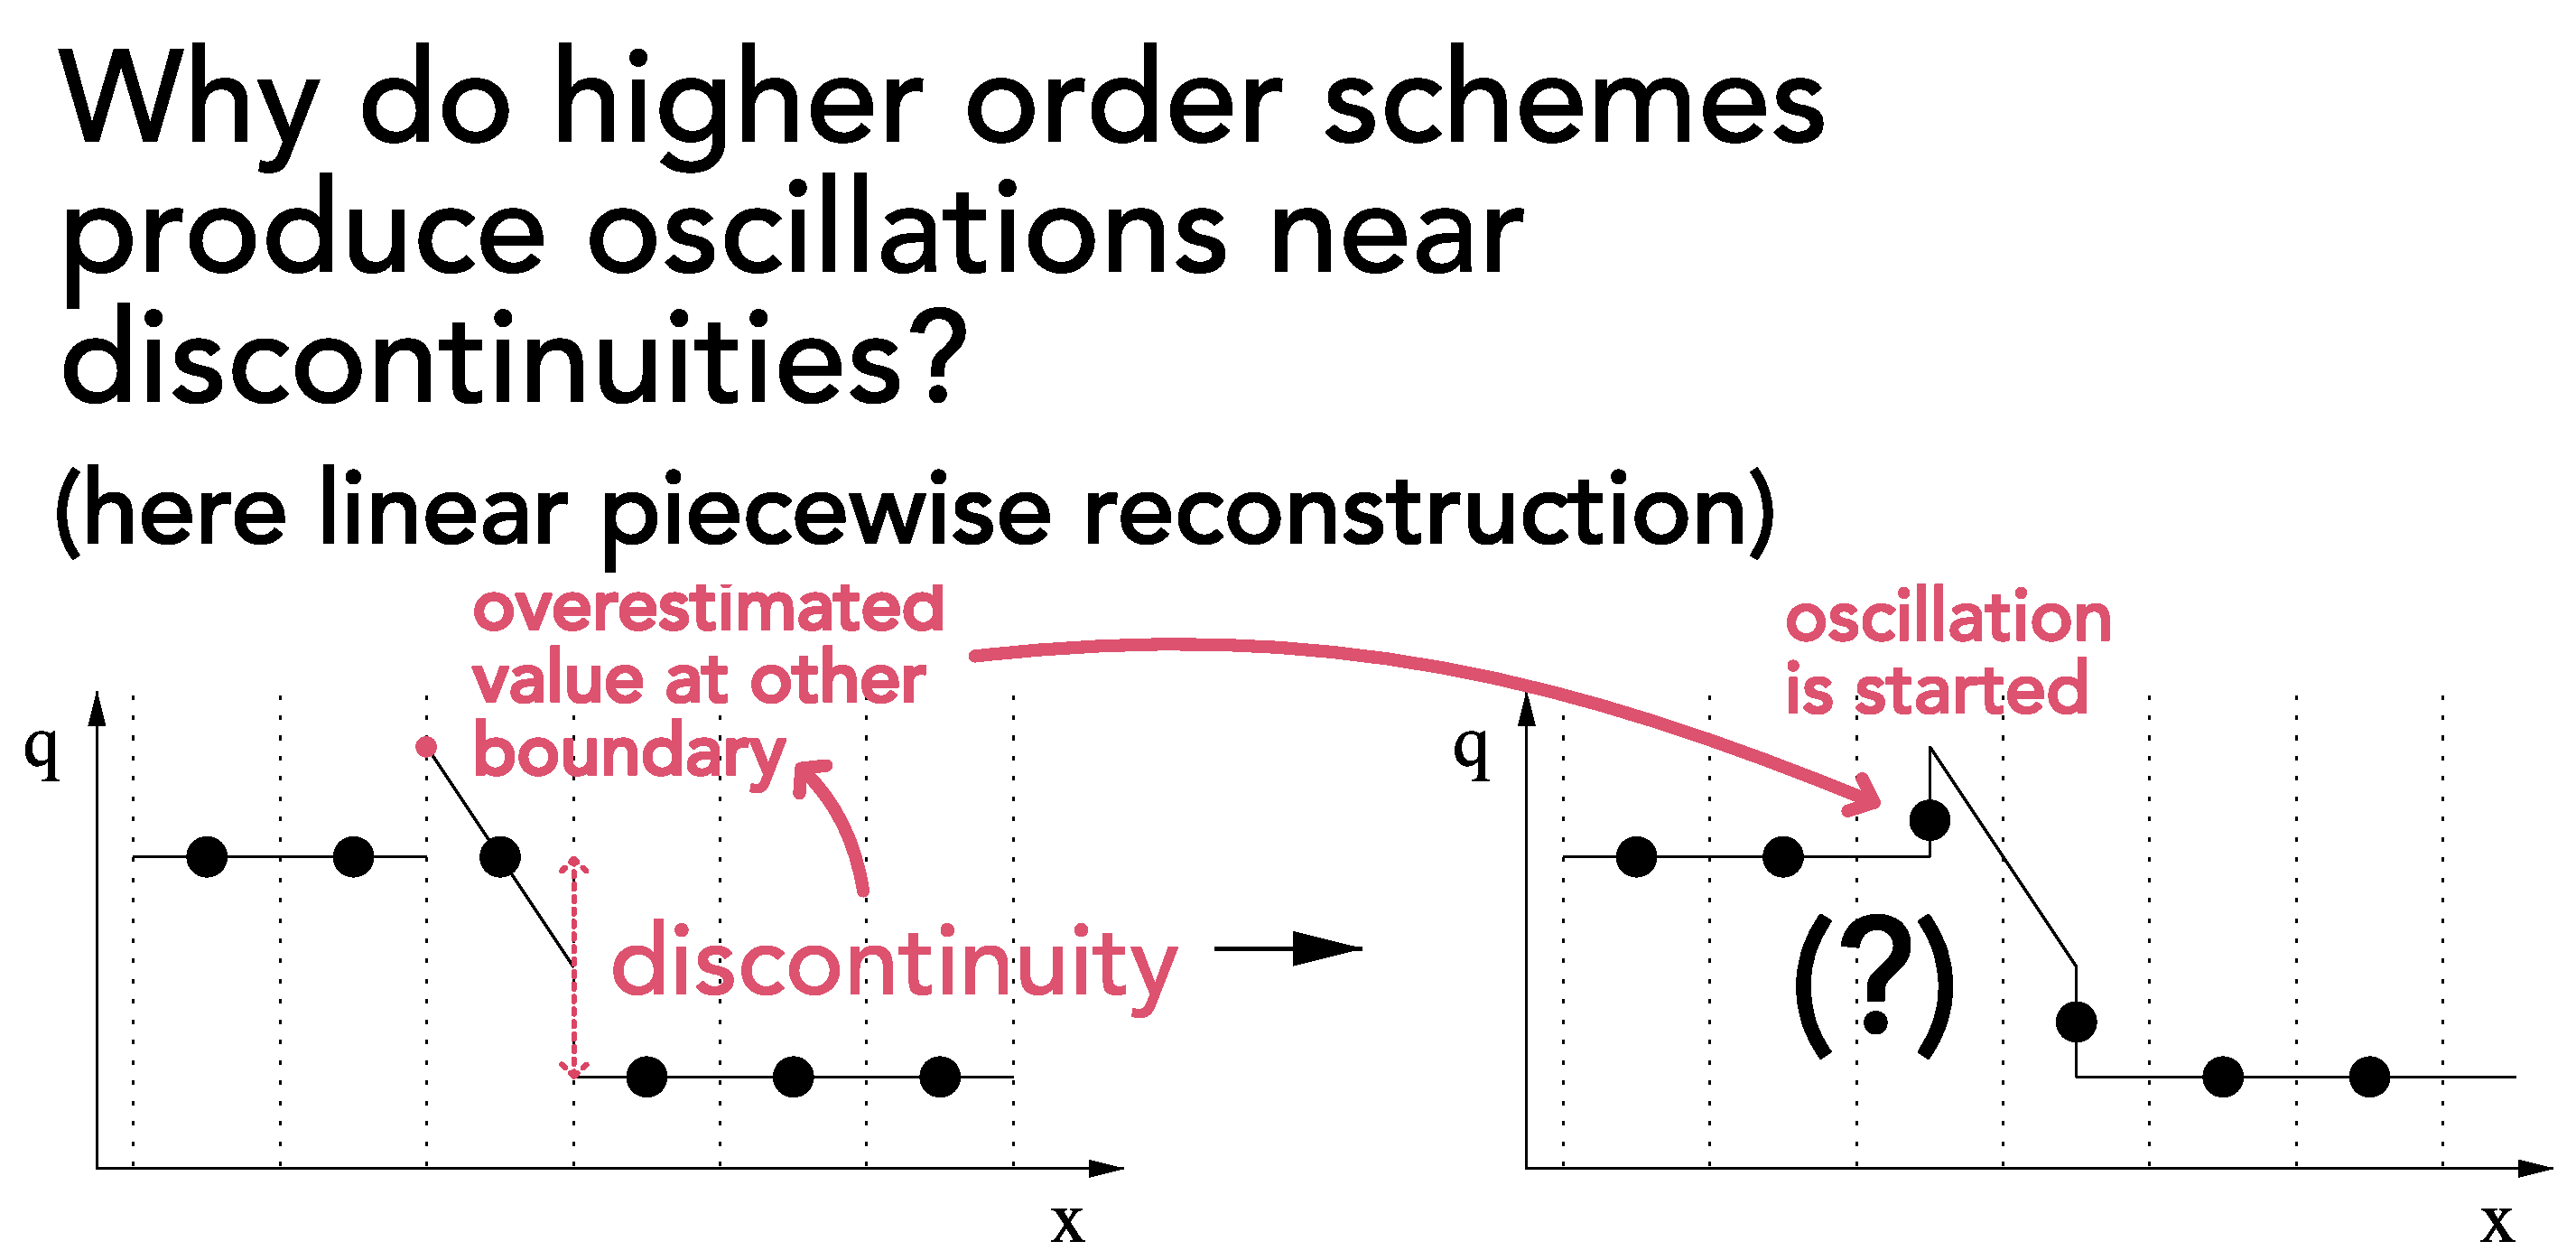
\includegraphics[width=0.8\textwidth]{figures/hoexp.pdf}
    \caption{Illustration of the principle of oscillations at discontinuities in higher order methods.}
    \label{fig:high_order_oscillations}
\end{figure}

\begin{table}[htb!]
    \centering
    \begin{tabular}{|p{0.45\textwidth}|p{0.45\textwidth}|}
        \hline
        \textcolor{green1}{Pro lower} & \textcolor{red1}{Con lower} \\
        \hline
        \begin{itemize}
            \item stable for complex flows
            \item no ocillations at discontinuities
            \item do not crash at high Mach numbers
        \end{itemize}
        &
        \begin{itemize}
            \item smear out solutions
            \item slower convergence to accurate solutions
            \item less accurate
        \end{itemize} \\
        \hline
    \end{tabular}
    \caption{Advantages and disadvantages of lower order methods.}
    \label{tab:low_order}
\end{table}

\subsection{Flux / slope limiters | adaptively switching between a high and low order method}
\problem{A system can contain very boring and strongly dynamic parts. It is very difficult to choose which solver is best for the global problem for all timesteps.}
\idea{Dynamically switch between orders and solvers. Use 2nd order where possible and 1st order where necessary (e.g. for discontinuities).}

Let us for simplicity consider a 1D problem with a single state variable $u$, e.g.
the viscous Burgers equation

\begin{equation}
    \partial_t u + \partial_x \left( \frac{1}{2} u^2 - \nu \partial_x u \right) = 0
\end{equation}

(which can be analytically solved using the Cole-Hopf transform $u = - 2 \nu \frac{1}{\phi} \partial_x \phi$\footnote{This is nice if we want to test different flux limiters against a ground-truth result.}).

Let $\mathcal{F}^H_{i+\frac{1}{2}}$ be a high-order flux computation and $\mathcal{F}^L_{i+\frac{1}{2}}$ be a low-order flux computation.
We use the flux
\begin{equation}
    \begin{gathered}
        F_{i+\frac{1}{2}}^{(n)}=\mathcal{F}_{i+\frac{1}{2}}^{L,(n)}\left(U_i, U_{i+1}\right)+\phi_{i+\frac{1}{2}}^{(n)}(r) \cdot\left(\mathcal{F}_{i+\frac{1}{2}}^{H,(n)}\left(U_i, U_{i+1}\right)-\mathcal{F}_{i+\frac{1}{2}}^{L,(n)}\left(U_i, U_{i+1}\right)\right) \\
        \text{high order for } \phi_{i+\frac{1}{2}}^{(n)}(r) = 1, \quad \text{low order for } \phi_{i+\frac{1}{2}}^{(n)}(r) = 0
    \end{gathered}
\end{equation}
with
\begin{equation}
    \begin{gathered}
        \text{flux limiter } \phi_{i+\frac{1}{2}}^{(n)}(r) \text{ based on the ratio } r = \frac{U_i - U_{i-1}}{U_{i+1} - U_{i}} \\
        \text{large if the jump of interest between } U_i \text{ and } U_{i+1} \\
        \text{ is large compared to the jump between } U_{i-1} \text{ and } U_{i}
    \end{gathered}
\end{equation}
with and exemplary flux limiter being
\begin{equation}
    \begin{gathered}
        \phi_{\text{minmod}} = \max(0, \min(1, r)), \quad r > 1 \rightarrow \phi_{\text{minmod}} = 1 \rightarrow \text{high order} \\
        \text{jumps of different sign} \quad \rightarrow \quad r \leq 0 \quad \rightarrow \quad \phi(r) = 0 \quad \rightarrow \quad \text{low order} \\
    \end{gathered}
\end{equation}
(illustrated in figure \ref{fig:minmod}) where it makes sense that for a big $r$ we use the higher order method: \textcolor{blue1}{If the jump between $i$ and $i+1$ is small compared to the jump between $i-1$ and $i$, we can assume that the solution is smooth and use the higher order method (no dicontinuity expected).}

\begin{figure}[htb!]
    \centering
    \includesvg[width=0.8\textwidth]{figures/minmod.svg}
    \caption{Minmod flux limiter.}
    \label{fig:minmod}
\end{figure}

The flux limiter concept is illustrated in figure \ref{fig:flux_limiter}.

\begin{figure}[htb!]
    \centering
    \includesvg[width=0.8\textwidth]{figures/flux_limiter.svg}
    \caption{Flux limiter concept.}
    \label{fig:flux_limiter}
\end{figure}

\yellowbox{\textbf{Why is $\phi$ called a flux limiter?} Higher order schemes can have larger slopes and predict larger fluxes, taking the lower order will has less of this problem.}

\subsubsection{Possibly advantageous properties of the flux limiter}
It is often advantageous for the limiters to be symmetric with the property
\begin{equation}
    \frac{\phi(r)}{r} = \phi \left( \frac{1}{r} \right)
\end{equation}
so that the switch works the same for forward and backward facing
gradients (mind the definition of $r$) (?).

Another property is based on the total variation
\begin{equation}
    \text{TV}(\vec{U}) = \sum_i \left| U_{i+1} - U_i \right|
\end{equation}
(where here $\vec{U}$ is the vector over the grid points not fluid variables),
called total variation diminishing (TVD) property
\begin{equation}
    \text{TV}(\vec{U}^{(n+1)}) \leq \text{TV}(\vec{U}^{(n)})
\end{equation}
which means no oscillation will appear but real ocscillations
in the system will also not grow but rather smeared out.
Minmod is TVD.

\pagebreak